\section{Searches for Specific Models}
\label{sec:stampCollecting}

Our signature, two isolated same-sign leptons plus, at least two b-tagged jets, and \met, 
is common to many different new physics scenarios.
Here we refine our analysis to define dedicated signal regions for a few of these scenarios,
and provide 95\% C.L. upper limits on their respective model parameter space.


\subsection{Same sign top production due to a $Z'$}
\label{sec:sstops}

This is an extension of the 2010 CMS published CMS analysis\cite{sstop}.
The main difference is that here in order to improve the signal-to-noise
we require two b-tagged jets.  This would not have made sense in 2010, since 
at the time the integrated luminosity was low enough that the analysis was almost
background free without requiring b-tags.

\subsubsection{Theoretical Discussion, $Z'$ model}

Recent measurements of the inclusive forward-backward $t\bar{t}$ production 
asymmetry ($A_{FB}$) from the 
Tevatron experiments show deviations from the standard model 
(SM) expectations~\cite{d0:fwtop, cdf:fwtop1, cdf:fwtop2}.
% The largest (3$\sigma$) deviation~\cite{cdf:fwtop2} is found 
% to be in the region of high invariant mass with $M_{t\bar{t}} >  450$ GeV. 
Several attempts have been made to explain this asymmetry~\cite{fcnczprime, Buckley, Gresham, zoltan}. 
One of the most natural ways to induce such an asymmetry would be through
Flavor Changing Neutral Currents (FCNC) in the top quark sector. 
The forward-backward asymmetry in $u\bar{u} \to t\bar{t}$ would then be generated
by t-channel exchange of a new massive $Z'$ boson that couples chirally to
$u$ and $t$ at the same vertex, as shown in Fig.~\ref{fig:ttbaras}~\cite{fcnczprime}.
The same type of interaction would also give rise to same-sign top pair production, 
as illustrated in Fig.~\ref{fig:tchannel} and Fig.~\ref{fig:schannel}. 
In this case, the initial state involves two $u-$quarks and 
thus the cross section at the LHC is enhanced due 
to the large valence quark parton density of the proton. 

\begin{figure}[htb]
\begin{center}
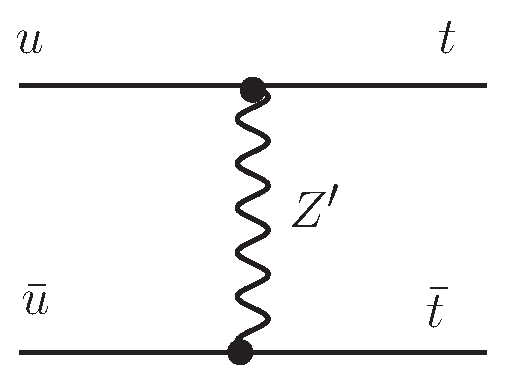
\includegraphics[width=0.35\linewidth, height=0.25\linewidth]{figs/ttbar_Z.pdf}
\caption{ Diagram for $t\bar{t}$ production induced by $Z'$ exchange which
can generate a forward-backward asymmetry. \label{fig:ttbaras}}
\end{center}
\end{figure}

\begin{figure}[htb]
\begin{center}
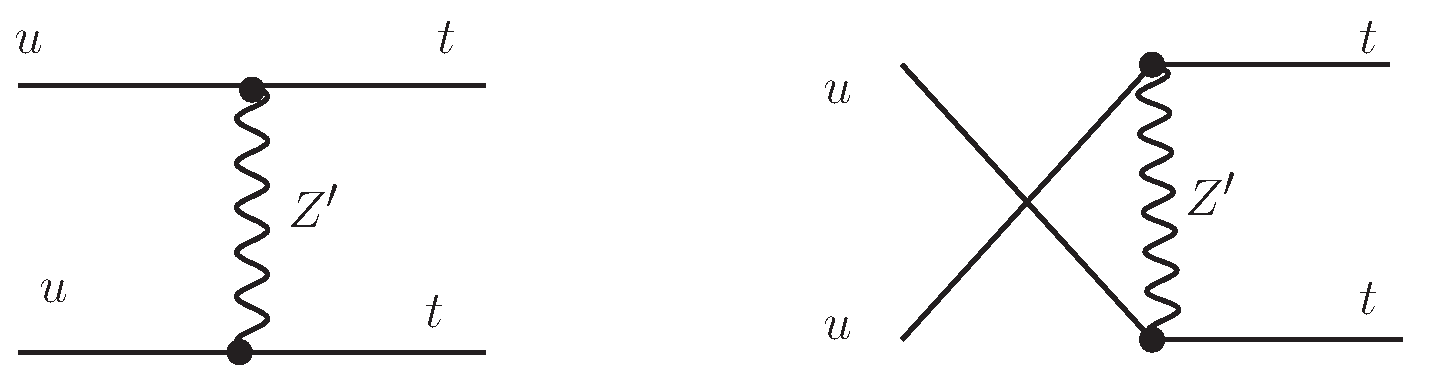
\includegraphics[width=0.7\linewidth, height=0.2\linewidth]{figs/sstop1.pdf}
\caption{ Diagrams for $tt$ pair production induced by $Z'$ exchange in the t-channel. 
\label{fig:tchannel}}
\end{center}
\end{figure}

\begin{figure}[htb]
\begin{center}
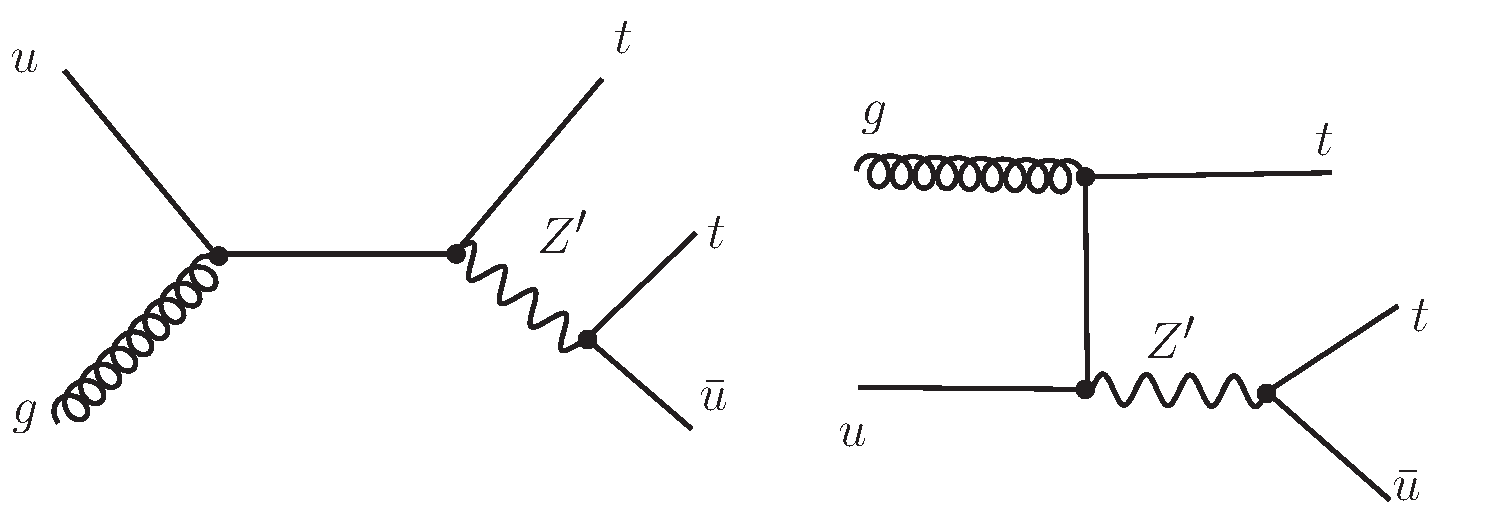
\includegraphics[width=0.7\linewidth, height=0.25\linewidth]{figs/sstop2.pdf}
\caption{ Diagrams for $tt\bar{u}$ production induced by $Z'$ exchange in the s-channel 
\label{fig:schannel}}
\end{center}
\end{figure}


We consider the model of Reference~\cite{fcnczprime}.  
The relevant $u-t-Z'$ interaction term in the Lagrangian is:

\begin{equation}
\label{eqn:L_berger}
  \mathcal{L} = g_W \bar{u} \gamma^\mu (f_L P_L + f_R P_R)tZ'_\mu + h.c
\end{equation}

where $g_W$ is the weak coupling strength. The left-handed coupling is set to $f_L = 0$, due 
to the $B_d-\bar{B_d}$ mixing constraint~\cite{Cao}. 
The right-handed coupling $f_R$ and the $Z'$ mass are free parameters in the model.
Within this model there is a narrow range of parameter space
consistent with the TeVatron measurements of $\sigma(p\bar{p} \to t\bar{t})$ 
and $A_{FB}$, which is not excluded by direct searches for same sign tops.
This region is illustrated in Fig.~\ref{fig:berger_limit}.

% Fig.~\ref{fig:tchannel} shows the t-channel exchange diagrams that can lead to the same-sign $tt$ final state. 
% As expected the coupling appears twice in the Feynman diagrams, thus the predicated rate is proportional to $f_R^4$. 

\begin{figure}[htb]
\begin{center}
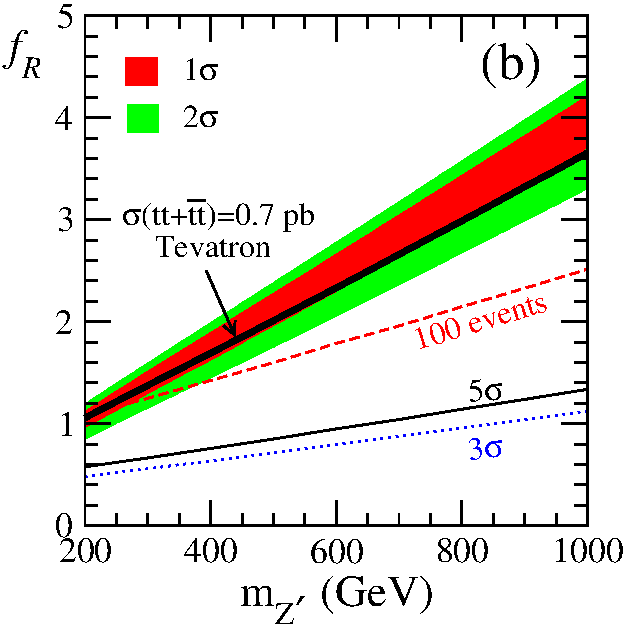
\includegraphics[width=0.4\linewidth]{figs/berger_limit.pdf}
\caption{\protect From Reference~\cite{fcnczprime}; the shaded area covers the parameter
space consistent with the $A_{FB}$ and $\sigma(t\bar{t})$ from the Tevatron;
The line indicated by the arrow shows the Tevatron limit inferred by the authors
from same sign top searches at the Tevatron; the remaining lines represent the
expectations of Reference~\cite{fcnczprime}.
for LHC searches in 1 fb$^{-1}$. \label{fig:berger_limit}}
\end{center}
\end{figure}

Monte Carlo events for this model were generated using Madgraph in the same way as 
for the 2010 analysis (see Reference~\cite{ttAN}).



\subsubsection{Signal region definition for same sign top from $Z'$}
\label{sec:sstopsigdefinition}
In this study we search for same-sign dileptons originating from $tt$ 
or $ttj$ pair production as described above.  At the LHC $uu \to tt$ 
dominates over $\bar{u}\bar{u} \to \bar{t}\bar{t}$, thus we concentrate
on same-sign positive leptons.  The \met~~and $H_T$ cuts are typical 
of a dilepton top analysis: two or more jets of $P_T>40$ GeV, 
$\met > 30$ GeV and $H_T > 80$ GeV.  This corresponds to Table~\ref{tab:yieldBase_pp}:
5 events observed and 4.42 $\pm$ 0.80 $\pm$ 1.39 expected from background.

\subsubsection{Limits on the $Z'$ model}
\label{sec:sstopslimits}
Using the results from Section~\ref{sec:sstopsigdefinition}, we set 
a limit at 95\% CL of 7.2 events using the CL$_{\rm S}$ method.
The expected limit is 6.4 events.
% $7.8^{+3.6}_{-3.1}$ events.
In the MC we find $Acc \times Eff \times BR = 0.00233$, independent of $Z'$ mass. 
This results in an upper limit on the cross-section of 0.67 pb.
The limit includes uncertainty
on JES (12\%), btagging (10\%), lepton efficiencies (11\%), luminosity (4.5\%),
and PDF (3\%).
Our limit is a factor of 25 more stringent than our
2010 result\cite{sstop} and also a factor of 5.5 better
than that of Atlas\cite{sstopatlas}.

The cross-section limit is turned into an exclusion limit in the $m(Z')$ vs $f_R$
plane using the LO calculation of the $pp \to tt$ cross-section in this model.
This is shown in Figure~\ref{fig:sstopexclusion}, together with the corresponding
plot from the 2010 analysis.  The region of parameter space consistent 
with the Tevatron measurements of $A_{FB}$ is excluded.


For $M_{Z'} >> M_{\rm top}$ the Lagrangian of equation 1 is 
equivalent to 
$\mathcal{L} = -\frac{1}{2}\frac{C_{RR}}{\Lambda^2}
 [\bar{u} \gamma^\mu t][\bar{u} \gamma_{\mu} t] + h.c.$~\cite{cdfth2},
with $\frac{C_{RR}}{\Lambda^2} = \frac{2 g_W^2 f_R^2}{M_{Z'}^2}$.
 Our limit on $f_R$, calculated for $M_{Z'}=2$ TeV, 
would then correspond to $\frac{C_{RR}}{\Lambda^2} < 0.6$ TeV$^{-2}$ at 
95\% confidence.  This is more stringent than the limit recently reported
by CDF: $\frac{C_{RR}}{\Lambda^2} < 3.7$ TeV$^{-2}$~\cite{cdflimit}.


\begin{figure}[htb]
\begin{center}
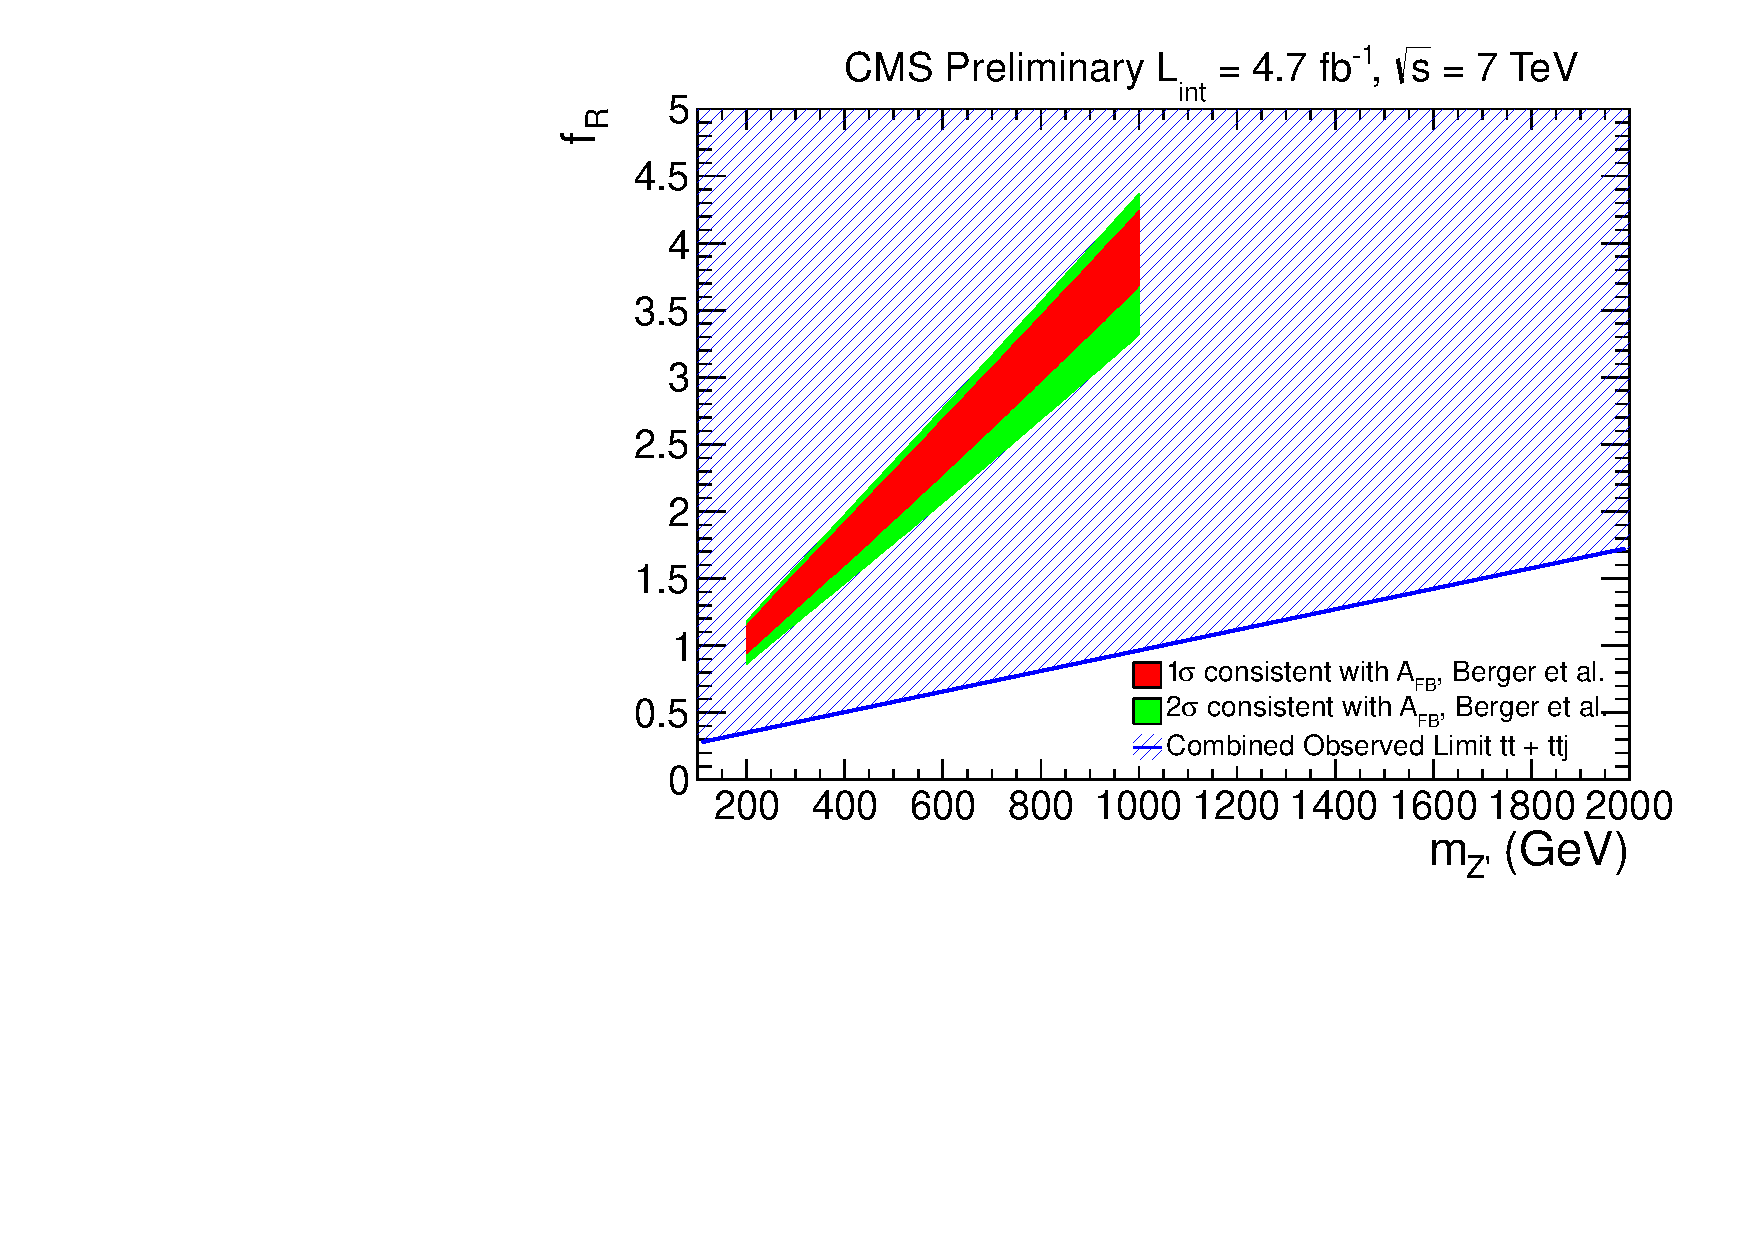
\includegraphics[width=0.45\linewidth]{figs/zprimecombined.pdf}
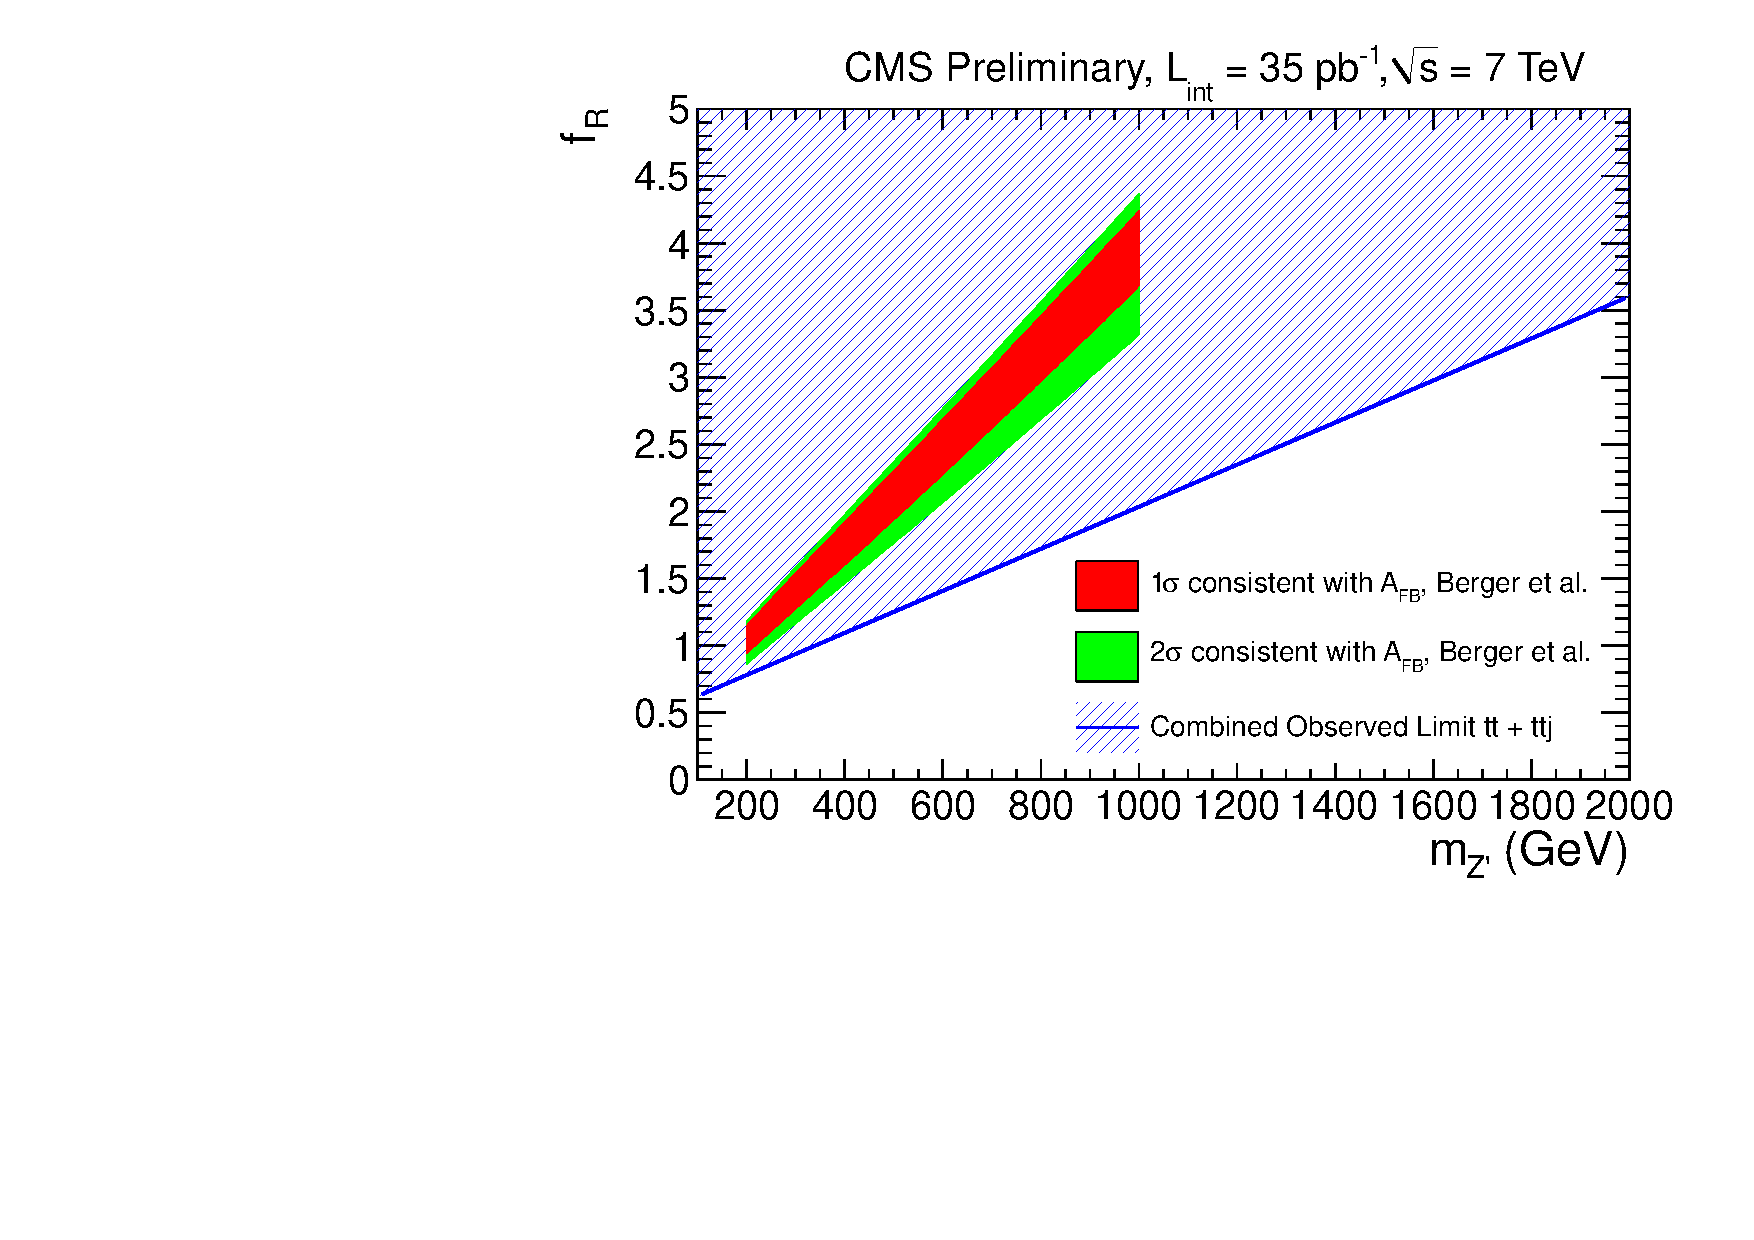
\includegraphics[width=0.45\linewidth]{figs/sscomb.pdf}
\caption{Exclusion regions from the 2011 analysis (left) and the 2010 analysis (right).
The exclusions are obtained using the LO cross-section for $tt$ production.  
Note that the cross-section is proportional to $f_R^4$.
\label{fig:sstopexclusion}}
\end{center}
\end{figure}

%\subsubsection{What is still missing for the $Z'$ model}
%\begin{itemize}
%\item Double check calculation of $\frac{C_{RR}}{\Lambda^2}$
%\item Double check acceptance numbers
%\end{itemize}


%\clearpage


\subsection{Maximally Flavor Violation Model (MXFV)}
\label{sec:mxfv}

\subsubsection{Theoretical discussion of MXFV}
\label{sec:mxfvtheory}

This is a model~\cite{mxflv1,mxflv2,mxflv3} with a new scalar 
SU(2) doublet field $\Phi_{FV} = (\eta^0,\eta^+)$ that couples the first and third 
generation quarks ($q_1,q_3$) via a Lagrangian term 
$\mathcal{L}_{FV} = \xi_{13} \Phi_{FV} q_1 q_3$.  Remarkably, it appears that this
model is largely consistent with constraints from flavor physics.

The model results in same sign top pairs in the final state as foolows
\begin{itemize}

\item Single $\eta^0$ production: $ug \to t\eta^0 \to tt\bar{u}, t\bar{t}u$

\item $\eta^0$ pair production: $u \bar{u} \to \eta^0 \eta^0 \to tt\bar{u}\bar{u},
uu\bar{t}\bar{t}, t\bar{t}u\bar{u}$

\item $\eta^0$ $t$-channel exchange: $uu \to tt$, $\bar{u}\bar{u} \to \bar{t}\bar{t}$
\end{itemize}

Monte Carlo events were generated using LHE files\cite{simplifiedModel} interfaced 
with Madgraph.  Madgraph was used to decay the top quarks in order to preserve 
spin-correlations.  The cross-sections at LO for same sign $tt$ pairs for the three
processes in the MXFV model is shown in Figure~\ref{fig:mxvxsec}.  The $t$-channel
process is the dominant for $\xi = 1$.  At smaller values of $\xi$, 
$ug \to \eta^0 \to tt\bar{u}$ becomes more important, since its cross-section 
varies as $\xi^2$, while in the $t$-channel case it goes as $\xi^4$.

\begin{figure}[htb]
\begin{center}
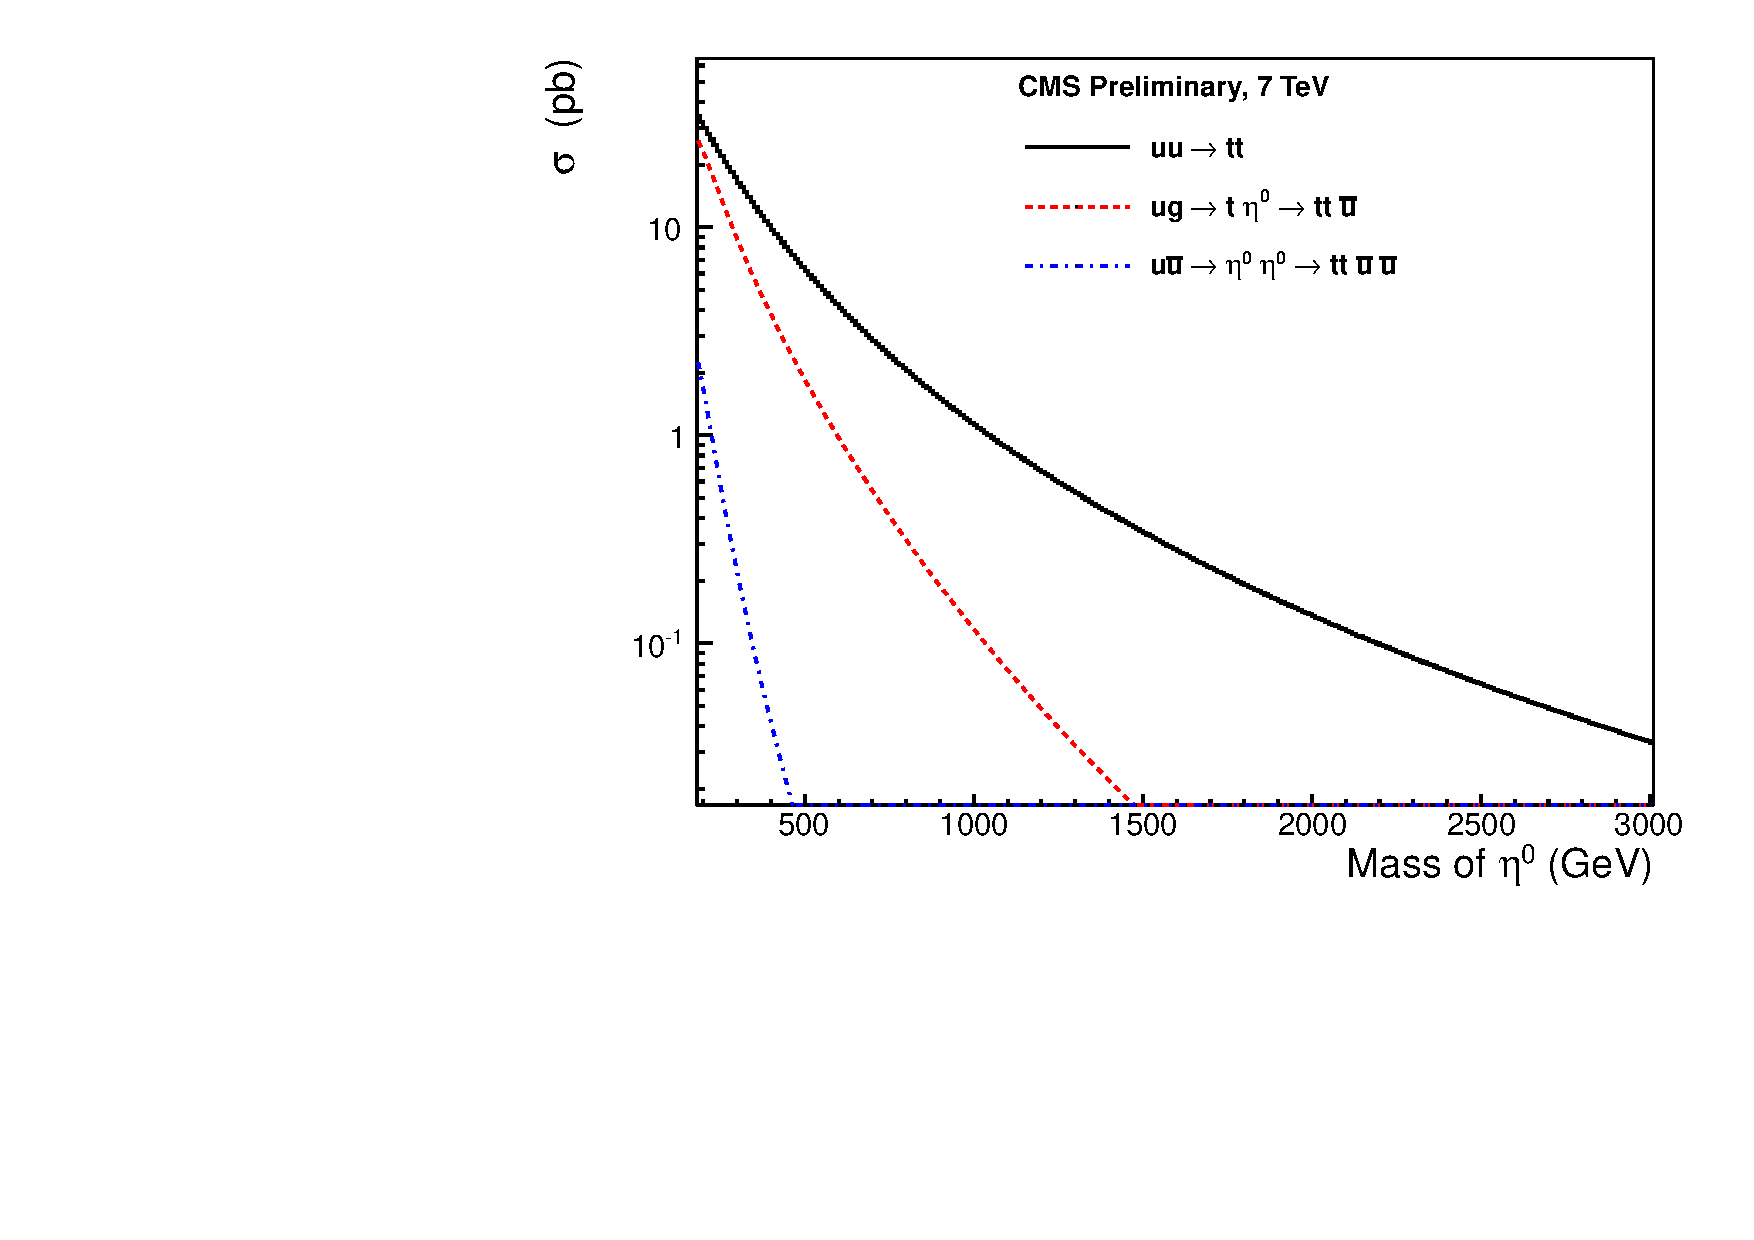
\includegraphics[width=0.55\linewidth]{figs/mxvxsec.pdf}
\caption{Cross section at LO for the $tt$ final state in the three MXFV modes
as a function of $\eta^0$ mass for $\xi = 1$.
\label{fig:mxvxsec}}
\end{center}
\end{figure}

\subsubsection{Signal region definition for the MXFV model}
\label{sec:mxfvdefinition}
The properties of the final state in this model are basically the same as in the $Z'$ model.
Thus, we use the same signal region definition (see Section \ref{sec:sstopsigdefinition}).


\subsubsection{Limits for the MXFV model}
\label{sec:mxfvlimits}
Our limits in the $\xi$-M($\eta^0$) plane are shown in 
Figure~\ref{fig:MxVExcl}.
They are calculated using the LO cross-section for this model.
Our limits are better than those of CDF\cite{mxflv3}.

\begin{figure}[htb]
\begin{center}
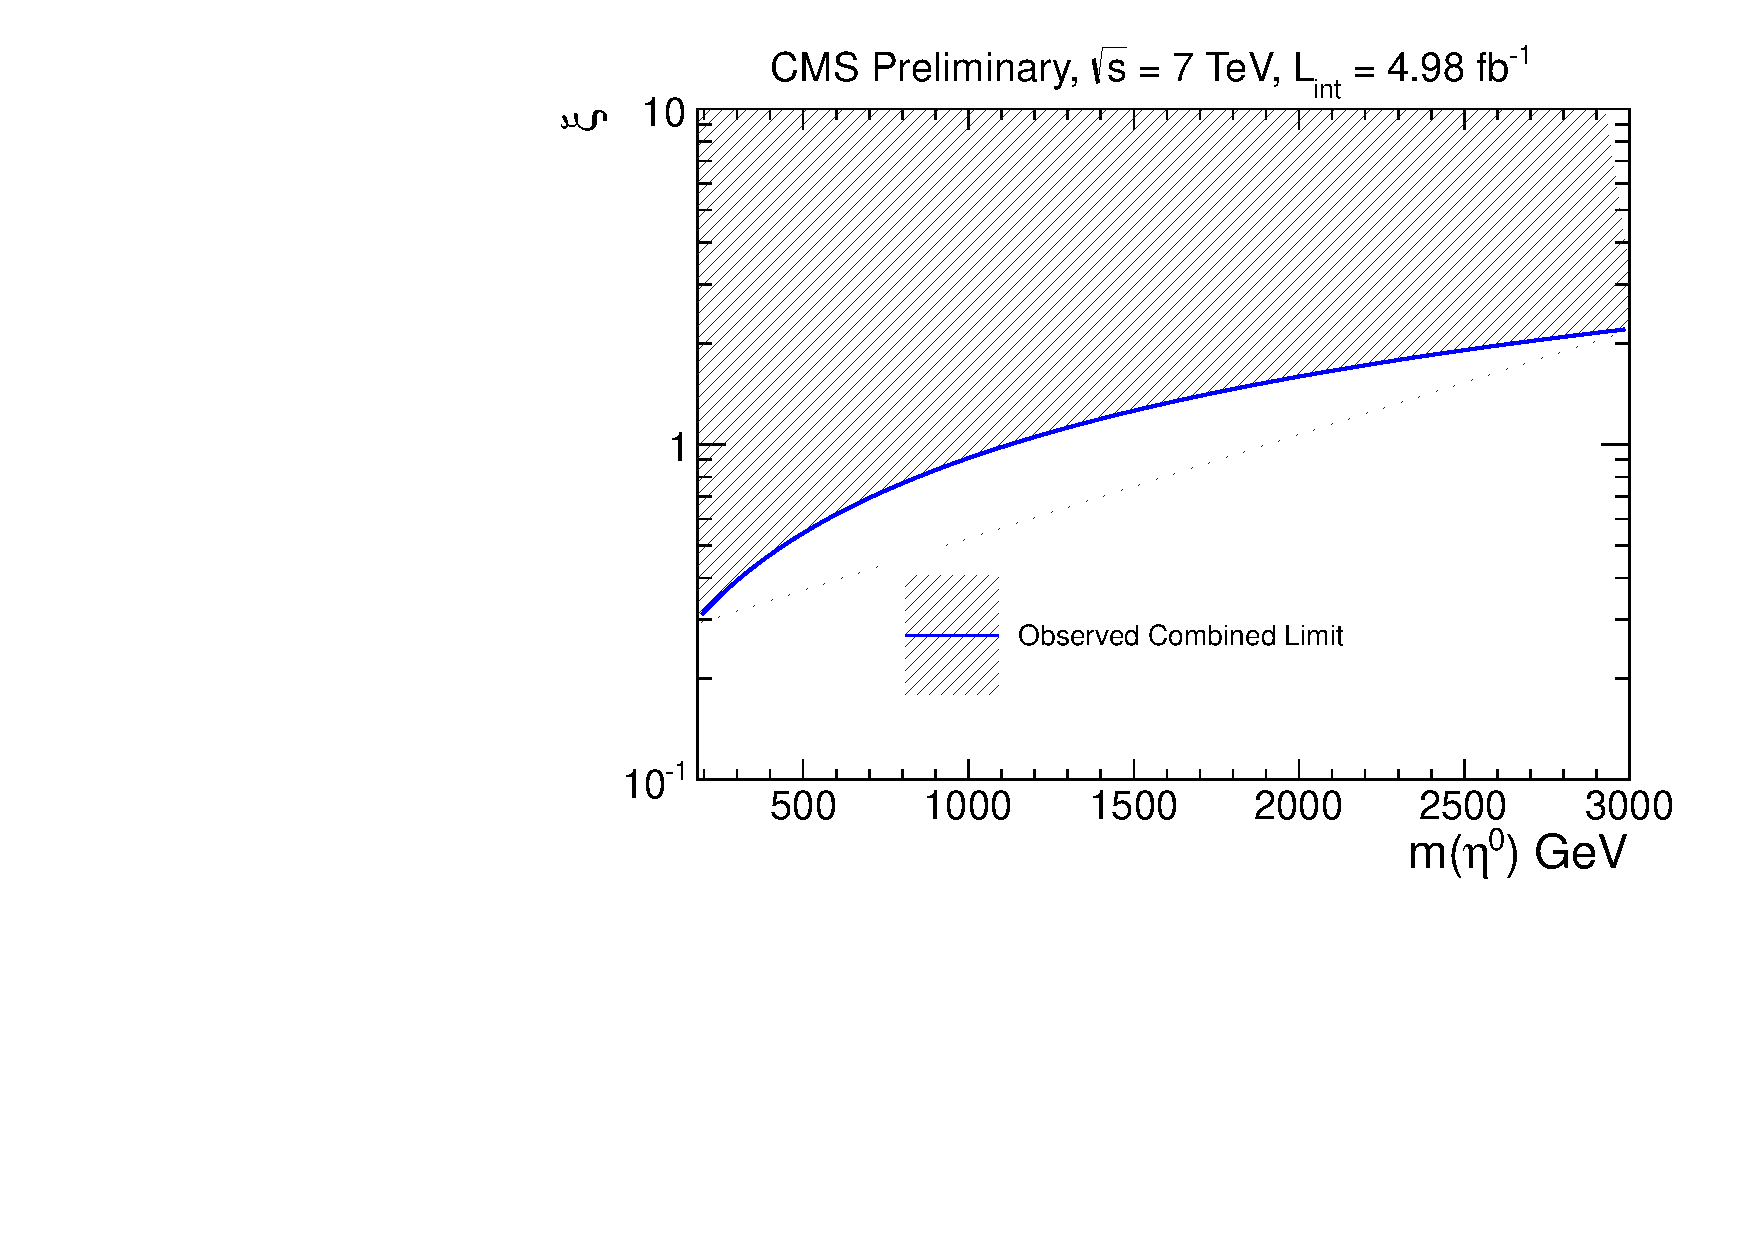
\includegraphics[width=0.45\linewidth]{figs/MxVExclCombined.pdf}
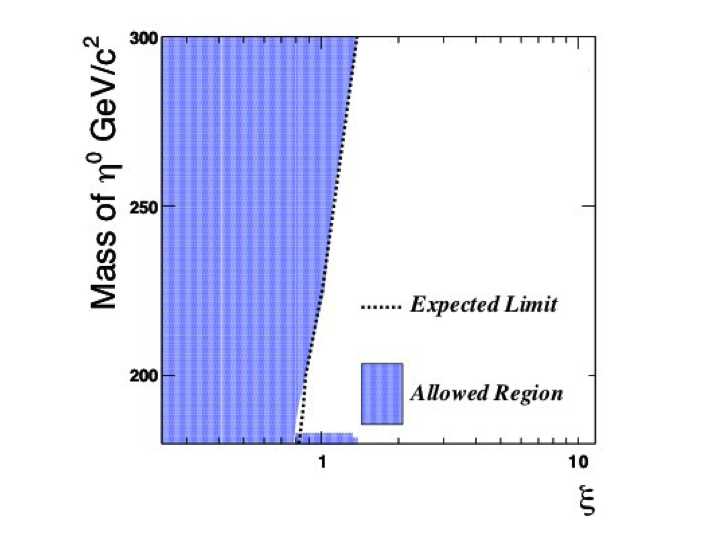
\includegraphics[width=0.45\linewidth]{figs/CDFlimit.png}
\caption{Limits in the $\xi$-Mass($\chi^0$) plane.  Left: CMS.  Right: CDF
\label{fig:MxVExcl}}
\end{center}
\end{figure}

%\subsubsection{What is still missing for the MXFV model}
%\begin{itemize}
%\item Need to include the $tt\bar{u}$ final state
%\item Rescale everything to take into account that the leptonic BR in MG is not quite right
%\item Signal Contamination effects (should be tiny)
%\item Prettify the exclusion plot, put CDF on same plot perhaps
%\end{itemize}



\subsection{$\widetilde{g} \to t\widetilde{t}$ Model}
\label{sec:firststopmodel}

\subsubsection{Theoretical discussion of the $\widetilde{g} \to t\widetilde{t}$ Model}
\label{sec:firststopmodeltheory}

This is an interesting model for stop pair production through gluino 
decays\cite{susyssbtags}\cite{susyssbtags2}\cite{wacker}\cite{naturalness4}.
It is a ``realistic'' and well-motivated 
model in the sense that it applies to the situation 
where all the squarks except the stop are very heavy.  A ``light'' stop is of course
generally favored in SUSY, and LHC results are pointing to ``heavy'' superpartners.
Then if the stop
is light enough the gluino would decay with 100\% BR as $\widetilde{g} \to t\widetilde{t}$
and then the stop would decay as $\widetilde{t} \to t \chi_1^0$, if kinematically 
accessible.
The parameters of the model are $M(\widetilde{g})$, $M(\widetilde{t})$, $M(\chi_1^0)$.

The final state after gluino pair production is then $tt\bar{t}\bar{t}\chi_1^0\chi_1^0$.
It is the same final state as the {\tt T1tttt} 
simplified model\cite{T1tttt}, except that 
it proceeds through an intermediate on-shell stop.  This final state is rich in leptons,
and has four b-quarks.  The same sign dilepton $+$ btags $+$ 
\met~~signature is a 
particularly good way to go after it.


\subsubsection{Signal region definition for the $\widetilde{g} \to t\widetilde{t}$ Model}
\label{sec:firststopdefinition}

\begin{figure}[htb]
\begin{center}
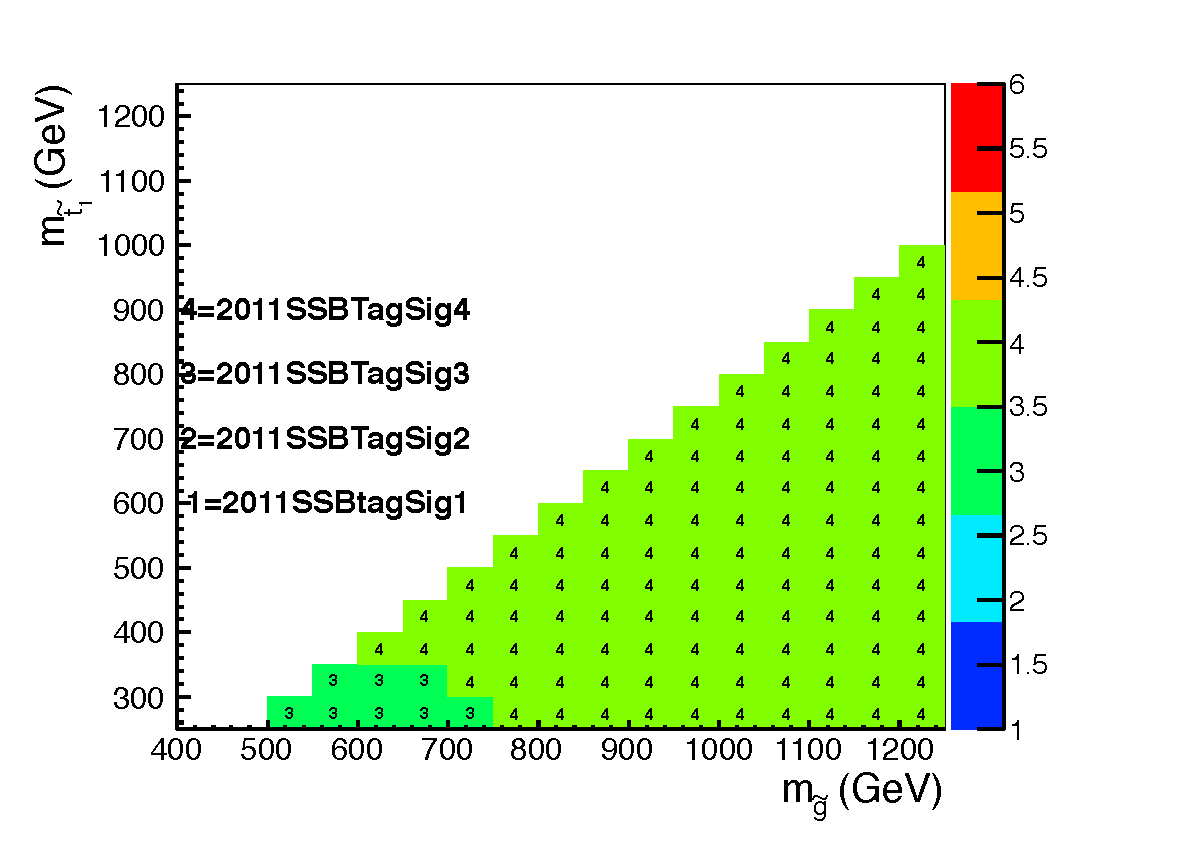
\includegraphics[width=0.65\linewidth]{figs/gluinostopsigreg.pdf}
\caption{The signal region with the best expected limit as a function of 
$m(\widetilde{g}$ vs. $m(\widetilde{t})$ plane for $m(\chi^0_1)$=50 GeV.
The coding is: 1=(200-50), 2=(200-150), 3=(320-50), and 4=(320-120), where
the first (second) number is the $H_T$ (\met) threshold in GeV. The number
of requested btags is 2 or more.
\label{fig:gluinostoptimize}}
\end{center}
\end{figure}


For each point in parameter space we use the signal region that gives
the best expected limit.  
{\bf (Note: so far the region with 3 btags has not been used).}
Limits are calculated using all experimental
uncertainties; the JES and btag uncertainties are calculated point-by-point.
An example of this optimization is shown in Figure~\ref{fig:gluinostoptimize},
where we show the choice of signal region that gives the best expected limit
in the $m(\widetilde{g})$ vs. $m(\widetilde{t})$ plane for the choice
$m(\chi^0_1)$=50 GeV.



%Using $\met > 50$ GeV and $H_T > 200$ GeV, which corresponds 
%to Table~\ref{tab:yield_ht200met50}: 5 events observed and 3.723 $\pm$ 0.787 $\pm$ 1.23 expected from backgrounds,
%we set a limit at 95\% CL of 7.65 events with the  CL$_{\rm S}$ method. The expected limit is 6.13. 

\subsubsection{Limits for the $\widetilde{g} \to t\widetilde{t}$ Model}
\label{sec:firststoplimits}



The limits on the production cross-section in this model in the 
gluino mass vs. stop mass plane for two choices of the 
LSP mass are shown in Figure~\ref{fig:mglinoStop}
Using the 
NLO$+$NLL cross-section for gluino pair production, we also place a limit
on the mass parameters of this model.  We basicaly can exclude 
$m(\widetilde{g})$ up to about 800 GeV for all kinematically allowed
values of the stop mass: 
$m(t)+m(\chi^0_1)~<~m(\widetilde{t})~<~m(\widetilde{g})-m(t)$. 



\begin{figure}[htb]
\begin{center}
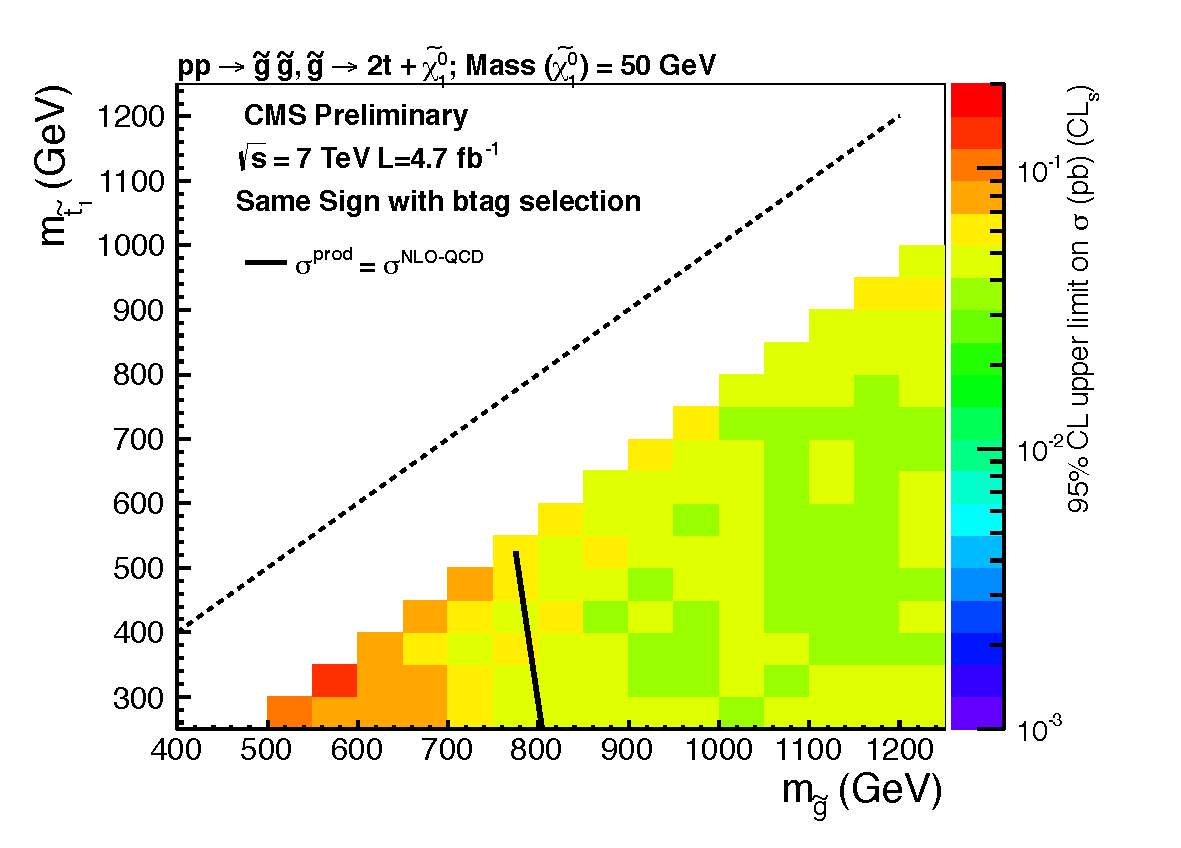
\includegraphics[width=0.47\linewidth]{figs/gluinostop50.pdf}
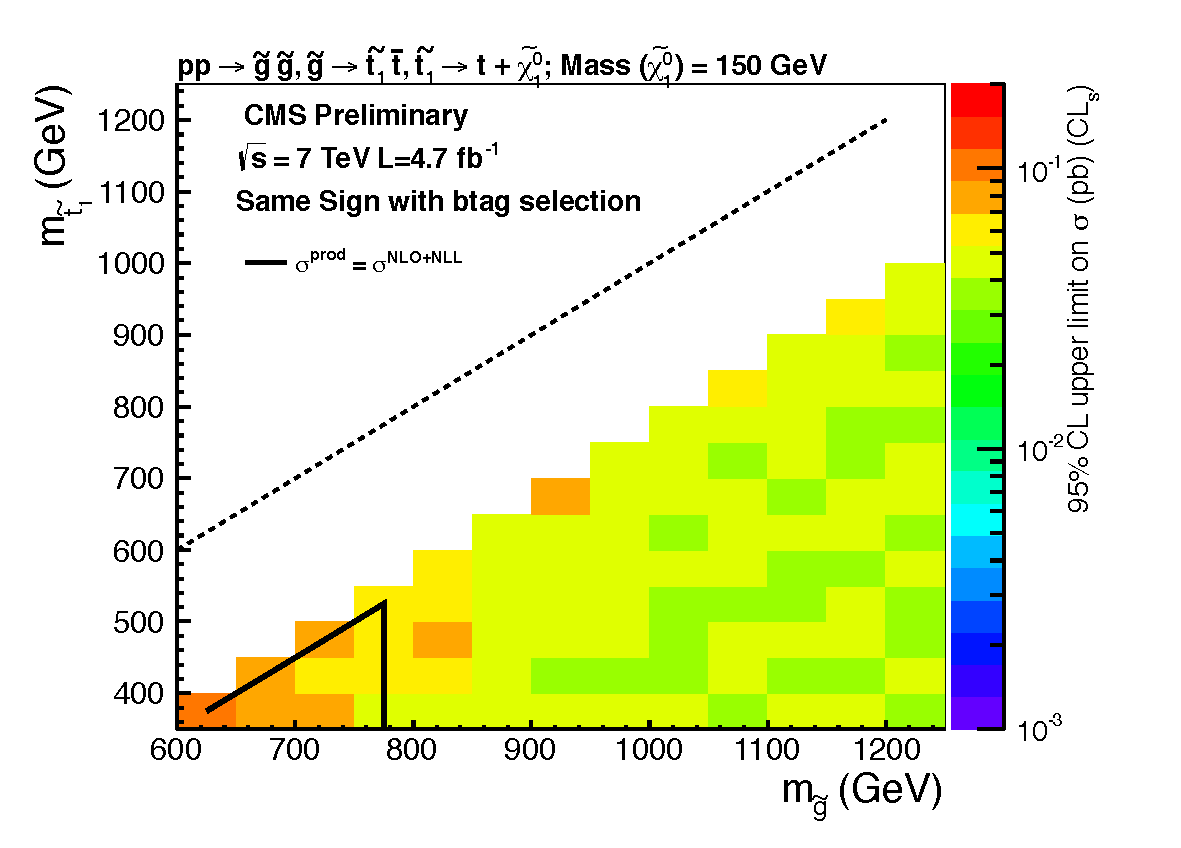
\includegraphics[width=0.47\linewidth]{figs/gluinostop150.pdf}
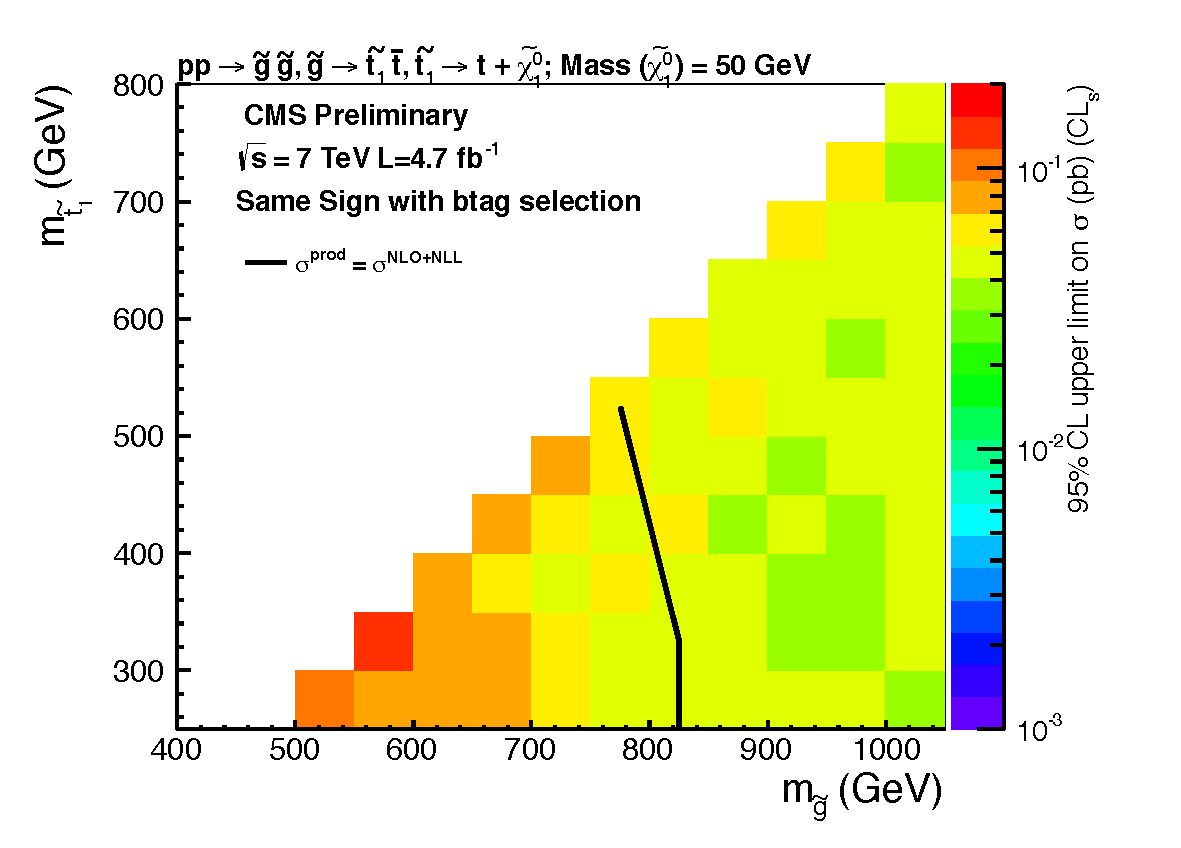
\includegraphics[width=0.47\linewidth]{figs/gluinostop50_zoom.pdf}
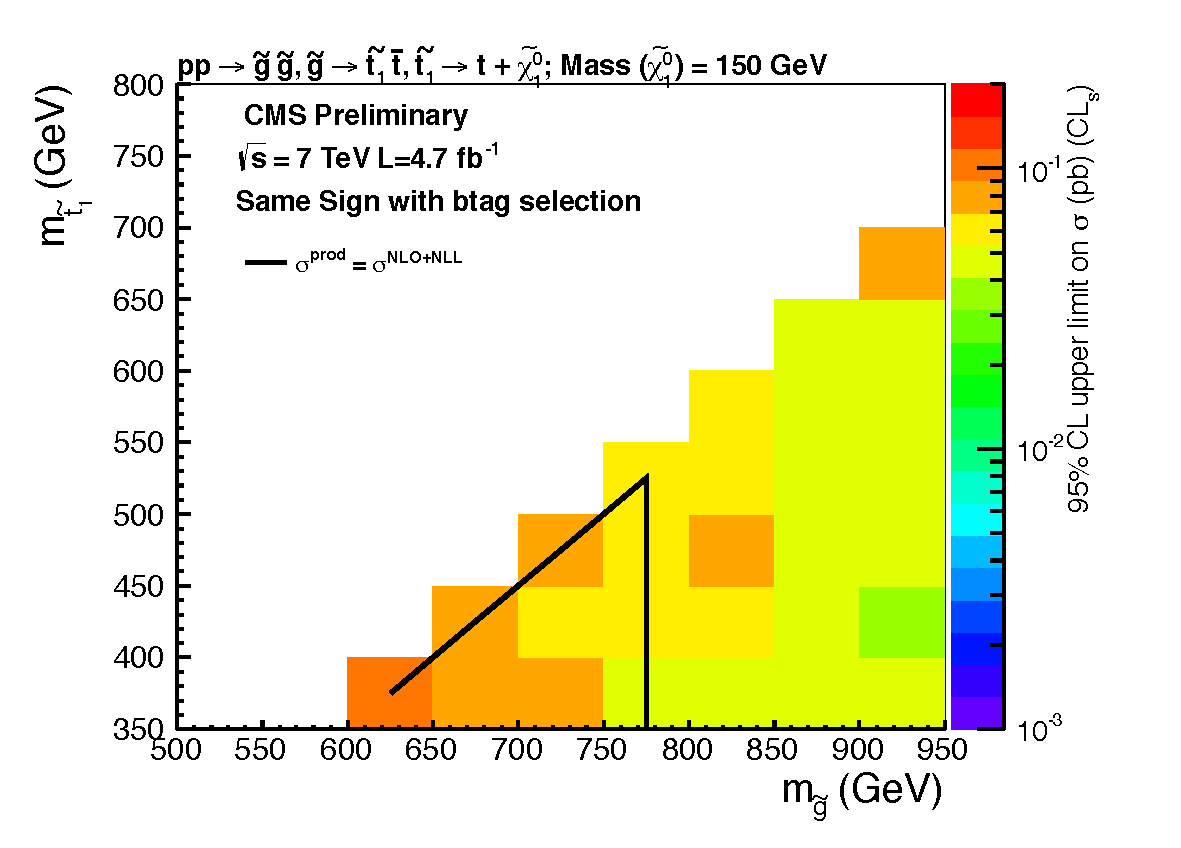
\includegraphics[width=0.47\linewidth]{figs/gluinostop150_zoom.pdf}
\caption{Cross section limits in the $m(\widetilde{g})$ vs. $m(\widetilde{t})$ plane
for $m(\chi_1^0)$ = 50 GeV (left) and 150 GeV (right).  
The bottom plots are versions of the top plots ``zoomed'' into the region
of interest.
\label{fig:mglinoStop}}
\end{center}
\end{figure}


%\subsubsection{What is missing for the $\widetilde{g} \to t\widetilde{t}$ Model}
%\begin{itemize}
%\item Perhaps more details on the MC signal generation???
%\item Need a reference for the {\tt T1tttt} model
%\item Maybe also a plot for LSP mass = 100 GeV? 
%\end{itemize}


\clearpage


\subsection{{\tt T1tttt} Model}
\label{t1ttmodel}

\subsubsection{Theoretical discussion of the {\tt T1tttt} Model}
\label{sec:t1tttheory}
The {\tt T1tttt} simplified model\cite{T1tttt} is very similar to the model of 
Section~\ref{sec:firststopmodel}.  In this model it is assumed that all squarks 
are very heavy, but the stop is somewhat lighter than the other 
quarks\cite{stopVirtual}\cite{stopVirtualPRD}.
Then the gluino would decay as $\widetilde{g} \to t\bar{t}\chi_1^0$ through virtual stops.
Other gluino decay modes would be suppressed because the stop is the lightest squark.
The final state after gluino pair production is $tt\bar{t}\bar{t}\chi_1^0\chi_1^0$,
just as in Section~\ref{sec:firststopmodel}.
The model parameters are $M(\widetilde{g})$ and $M(\chi_1^0)$.



\subsubsection{Signal region definition for the {\tt T1tttt} Model}
\label{sec:t1ttttdefinition}
For each point in parameter space we use the signal region that gives
the best expected limit, see Figure~\ref{fig:t1tttoptimize}.
{\bf (Note: so far the region with 3 btags has not been used).}
The limits include all experimental 
uncertainties.   The JES and btag uncertainties are calculated point-by-point.


\begin{figure}[htb]
\begin{center}
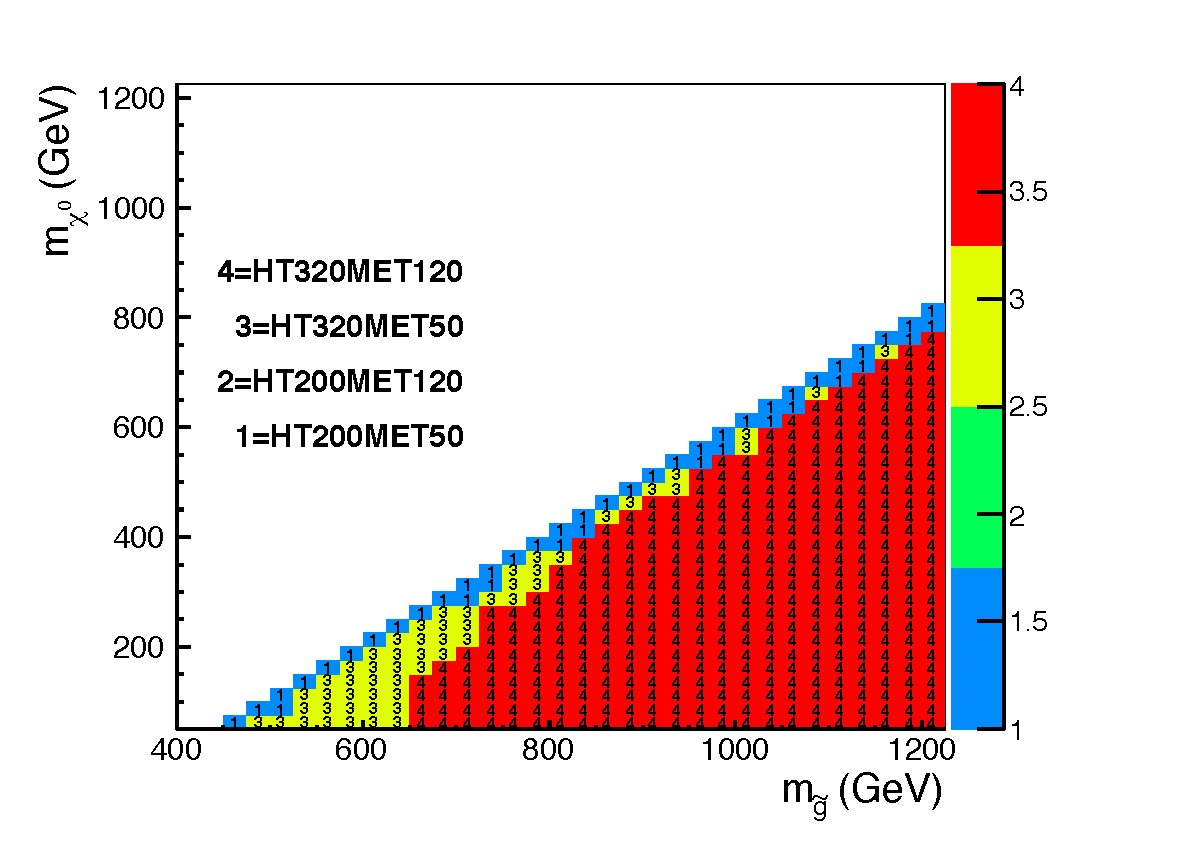
\includegraphics[width=0.4\linewidth]{figs/t1ttttsigreg.pdf}
\caption{The signal region with the best expected limit as a function of 
$m(\widetilde{g})$ vs. $m(\widetilde{t})$ plane for $m(\chi^0_1)$=50 GeV.
The coding is: 1=(200-50), 2=(200-150), 3=(320-50), and 4=(320-120), where
the first (second) number is the $H_T$ (\met) threshold in GeV. The number
of requested btags is 2 or more.
\label{fig:t1tttoptimize}}
\end{center}
\end{figure}


\subsubsection{Limits for the {\tt T1tttt} Model}
\label{sec:t1ttttlimits}
The limit on the production cross-section in this model in the 
gluino mass vs. LSP mass plane shown in Figure~\ref{fig:T1ttttLimit}.  
Using the 
NLO$+$NLL cross-section for gluino pair production, we place a limit
on the mass parameters as shown in Figure~\ref{fig:T1ttttLimit}.
Basically we exclude 
$m(\widetilde{g})$ up to about 800 GeV with a small dependence on 
$m(\chi_1^0)$.

\begin{figure}[htb]
\begin{center}
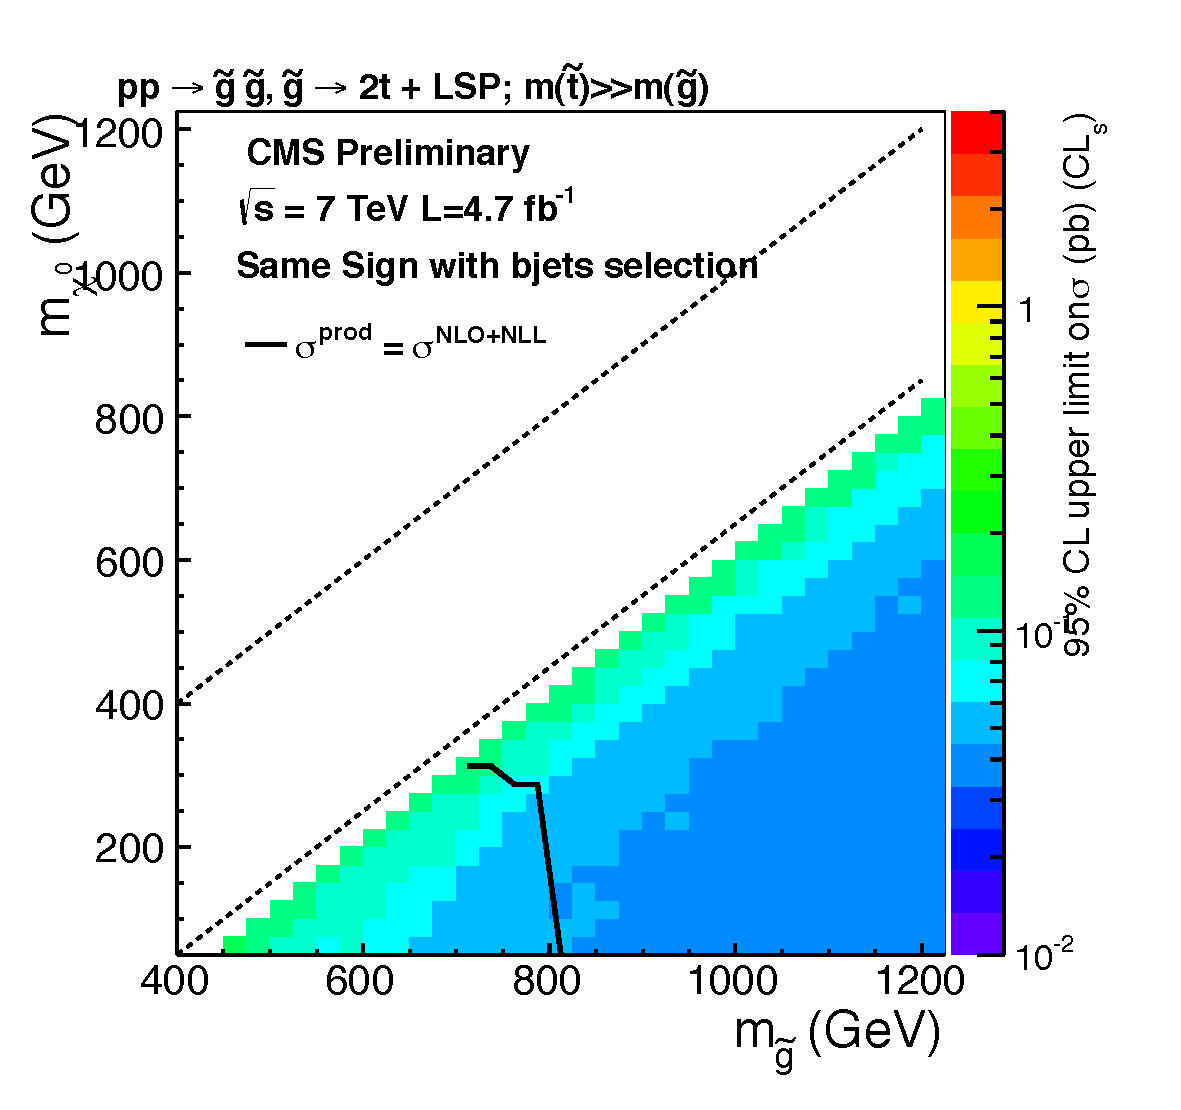
\includegraphics[width=0.48\linewidth]{figs/T1tttt.pdf}
\caption{Cross section limits in the $m(\widetilde{g})$ vs. $m(\chi_1^0)$ plane for the
{\tt T1tttt} model.  
\label{fig:T1ttttLimit}}
\end{center}
\end{figure}

%\subsubsection{What is missing for the {\tt T1tttt} Model}
%\begin{itemize}
%\item Need at least a sentence to say something which signal region contributes.  Or a plot.
%\item Need a reference for the {\tt T1tttt} model
%\end{itemize}


\clearpage

\subsection{Sbottom pair production model}
\label{sec:sbottompair}
In this model we have $pp \to \tilde{b}\tilde{b}$.  The sbottom decays 
as $\tilde{b} \to t\chi^{-}$ followed by $\chi^{-} \to W^- \chi_1^0$. 
The final state is $t\bar{t}W^+W^- \chi_1^0 \chi_1^0$. 
The model parameters are $M(\widetilde{b})$, $M(\chi_1^0)$, and $M(\chi^{\pm})$.
For simplicity we only consider mass parameters such that the $\chi^{-}$ is on shell.

\subsubsection{Signal region definition for the sbottom pair production model}
\label{sec:sbottompairdefinition}
For each point in parameter space we use the signal region that gives
the best expected limit, see Figure~\ref{fig:sbottomoptimize}.
{\bf (Note: so far the region with 3 btags has not been used).}
The limits include all experimental 
uncertainties.   The JES and btag uncertainties are calculated point-by-point.


\begin{figure}[htb]
\begin{center}
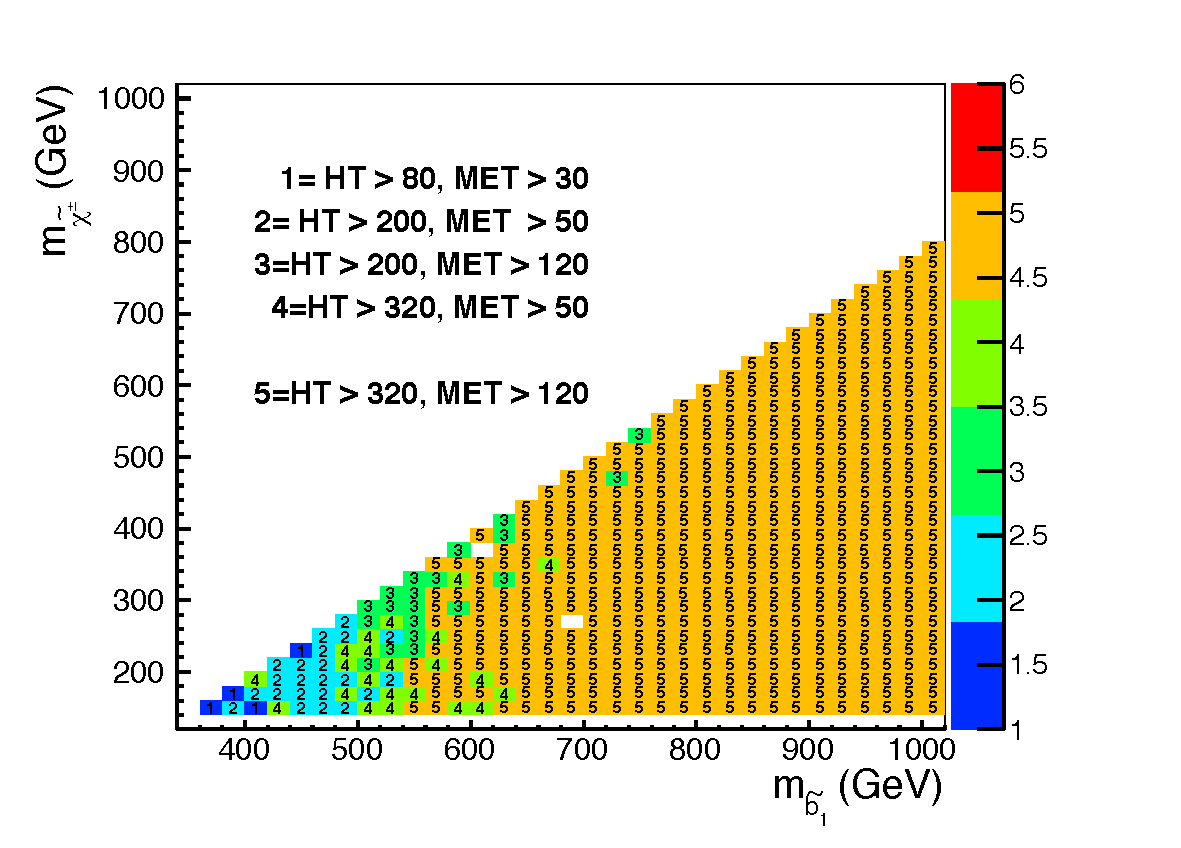
\includegraphics[width=0.5\linewidth]{figs/sbottom_regions.pdf}
\caption{The signal region with the best expected limit as a function of 
$m(\chi^{\pm}))$ vs. $m(\widetilde{b})$ plane for $m(\chi^0_1)$=50 GeV.
The coding is: 1=(80,30),
2=(200-50), 3=(200-150), 4=(320-50), and 5=(320-120), where
the first (second) number is the $H_T$ (\met) threshold in GeV. The number
of requested btags is 2 or more.
\label{fig:sbottomoptimize}}
\end{center}
\end{figure}


\subsubsection{Limits for the sbottom pair production model}
\label{sec:sbottompairlimits}
The limit on the production cross-section in this model in the 
sbottom mass vs. $\chi^{\pm}$ mass plane shown in 
Figure~\ref{fig:sbottomLimit} for 
$m(\chi^0_1)$=50 GeV. 
Using the 
NLO$+$NLL cross-section for gluino pair production, we place a limit
on the mass parameters as shown in Figures~\ref{fig:sbottomLimit}
and~\ref{fig:sbottomLimit1d}.
% We have little sensitivity to the model parameters.
% exclude $m(\widetilde{b})$ up to about 450 GeV for all
% kinematically allowed values of the chargino mass:
% $m(\chi^{\pm})~<~m(\widetilde{b})-m(t)$.

\begin{figure}[htb]
\begin{center}
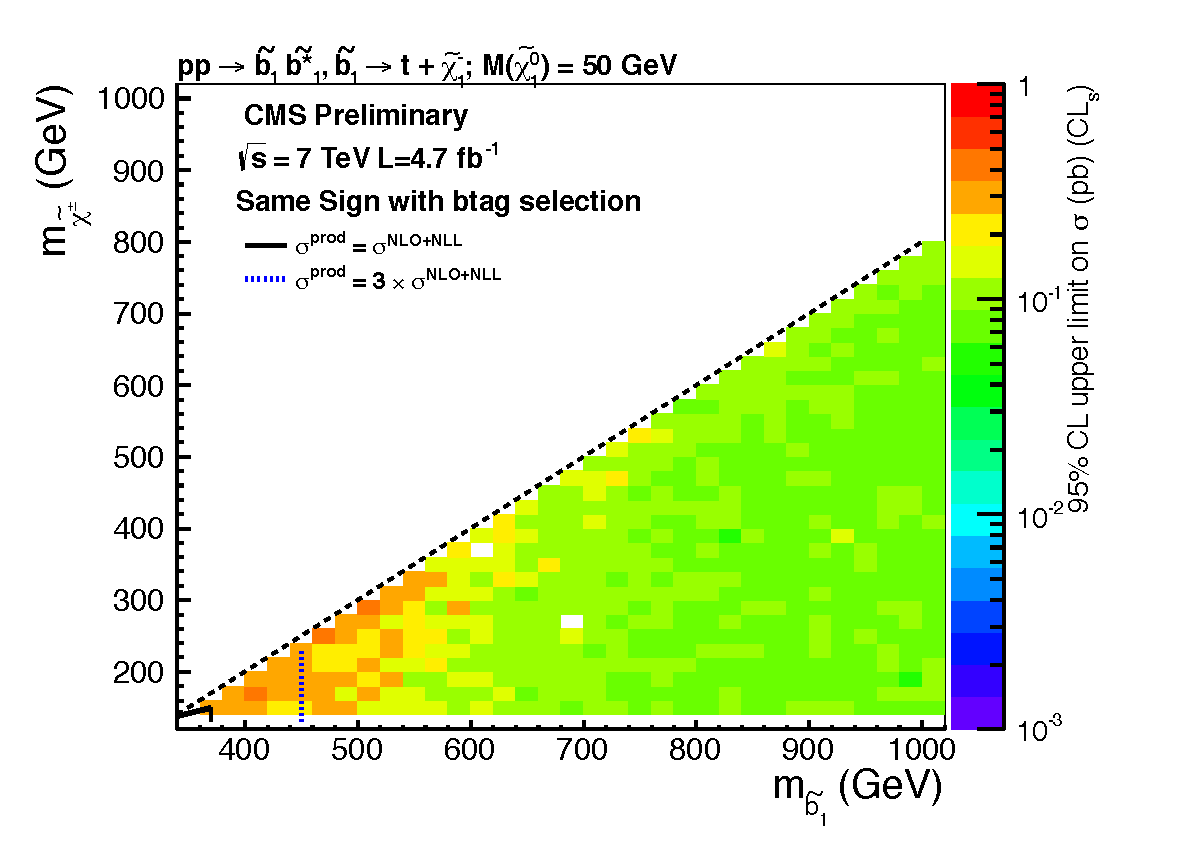
\includegraphics[width=0.48\linewidth]{figs/sbottom_limit.pdf}
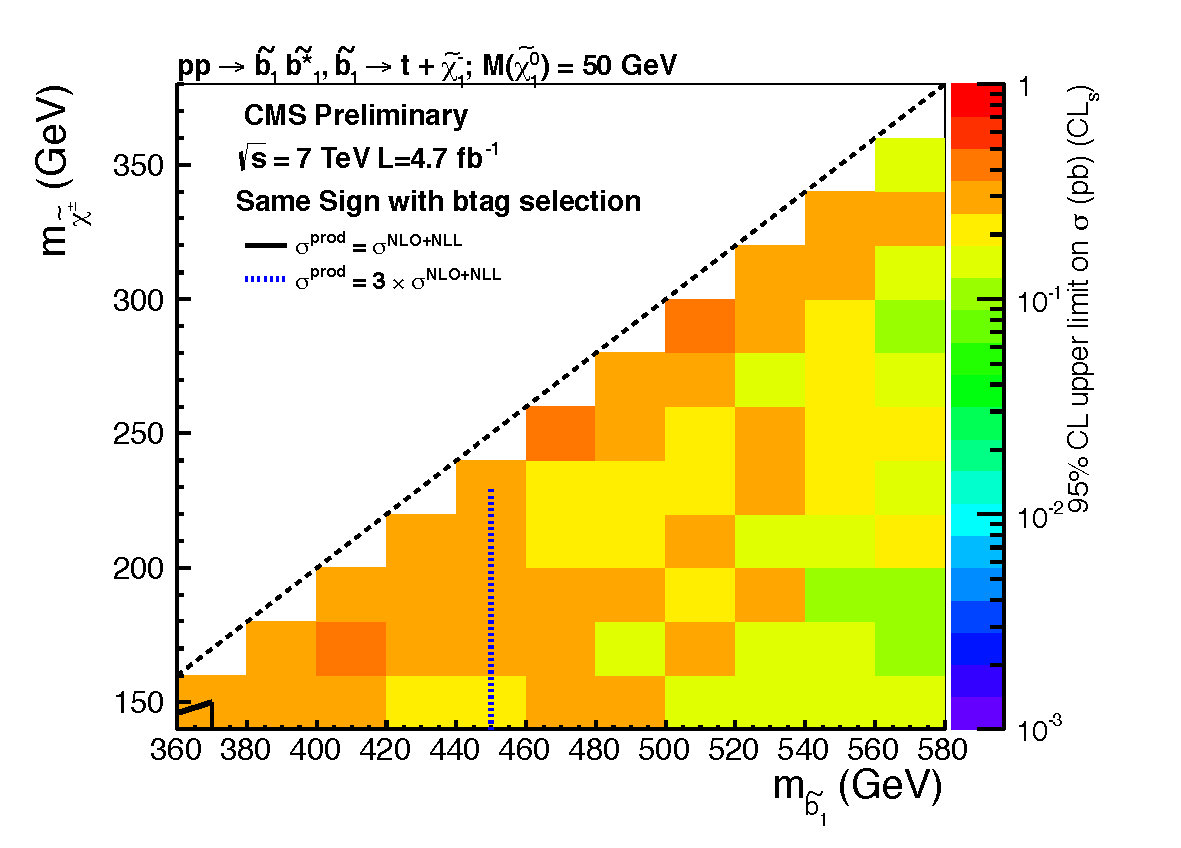
\includegraphics[width=0.48\linewidth]{figs/sbottom_limit_zoom.pdf}
\caption{Cross section limits in the $m(\widetilde{b})$ vs. $m(\chi^{\pm})$ 
plane for the sbottom pair production model with 
$m(\chi^0_1)$=50 GeV.  The rigth plot is a ``zoomed'' in version 
of the left plot.  This plot will be remade and zoomed in even 
further with more model points near the limit curve.\label{fig:sbottomLimit}}
\end{center}
\end{figure}


\begin{figure}[htb]
\begin{center}
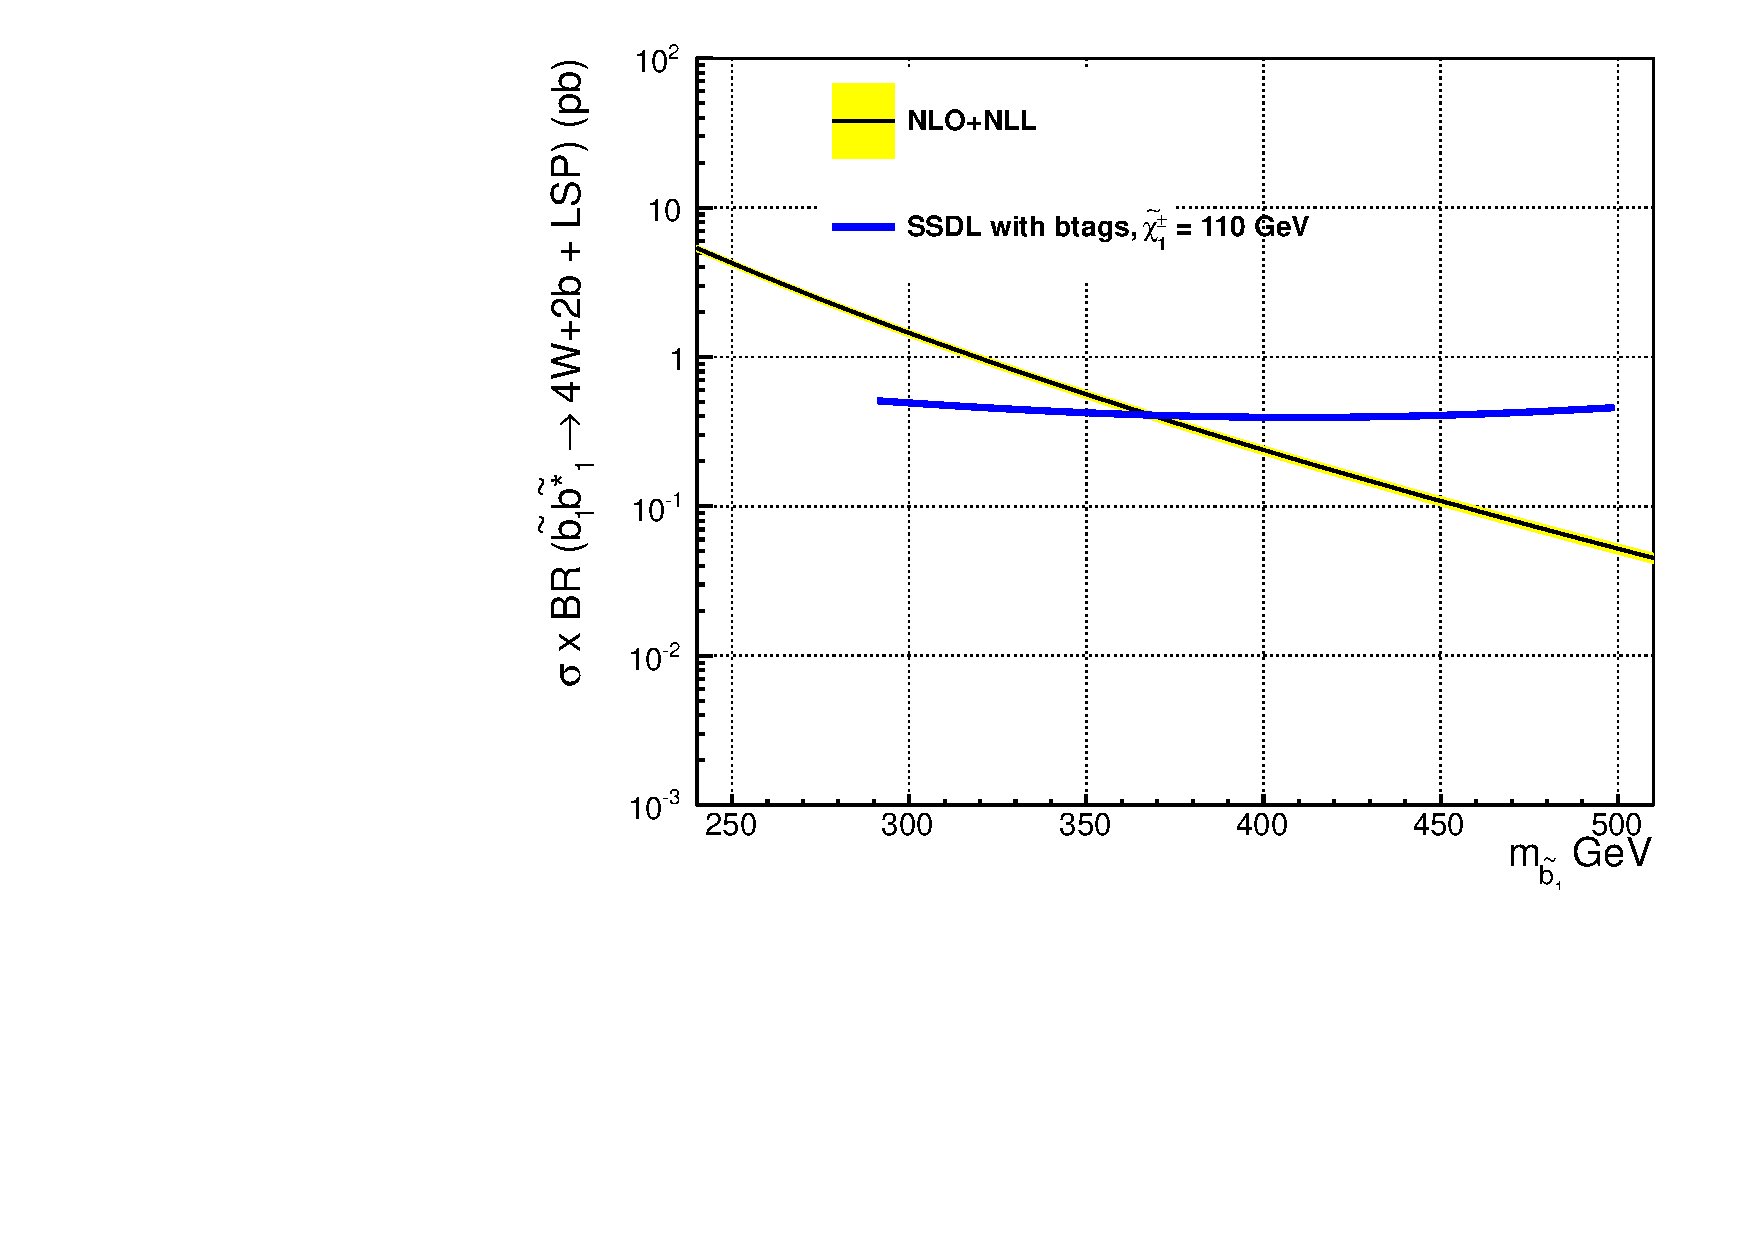
\includegraphics[width=0.48\linewidth]{figs/sbottom_1d.pdf}
\caption{Cross section limits as a function of sbottom mass
in the sbottom pair production model, compared with the 
sbottom pair-production coss-section.\label{fig:sbottomLimit1d}}

\end{center}
\end{figure}





%\subsubsection{What is missing for the sbottom pair production model}
%\begin{itemize}
%\item Everything in Sections~\ref{sec:sbottompairdefinition} and \ref{sec:sbottompairlimits}
%\item It would be nice to have a reference.  I am not sure that the references that
%we have on our twiki are appropriate. 
%\item Perhaps more details on the MC signal generation
%\end{itemize}



\subsection{$\widetilde{g} \to \widetilde{b}b$ Model}
\label{sec:gbb}
This model is mostly gluino pair production followed by 
$\widetilde{g} \to \widetilde{b}b$, $\widetilde{b} \to t \chi^{-}$ and
$\chi^{-} \to W^- \chi_1^0$. 
The final state is $t\bar{t}b\bar{b}W^+W^- \chi_1^0 \chi_1^0$
or $ttb\bar{b}W^+W^- \chi_1^0 \chi_1^0$ $(+ c.c.)$.
The model also includes the $b g \to \widetilde{b} \widetilde{g}$ process,
in which case the final state is
$tb\bar{b}W^+W^- \chi_1^0 \chi_1^0$ $(+ c.c.)$. 
The model parameters are $M(\widetilde{g})$
$M(\widetilde{b})$, $M(\chi_1^0)$, and $M(\chi^{\pm})$.
For simplicity we only consider mass parameters such that the $\chi^{-}$ is on shell.

\subsubsection{Signal region definition for the $\widetilde{g} \to \widetilde{b}\bar{b}$ Model}
\label{sec:gbbdefinition}

\begin{figure}[htb]
\begin{center}
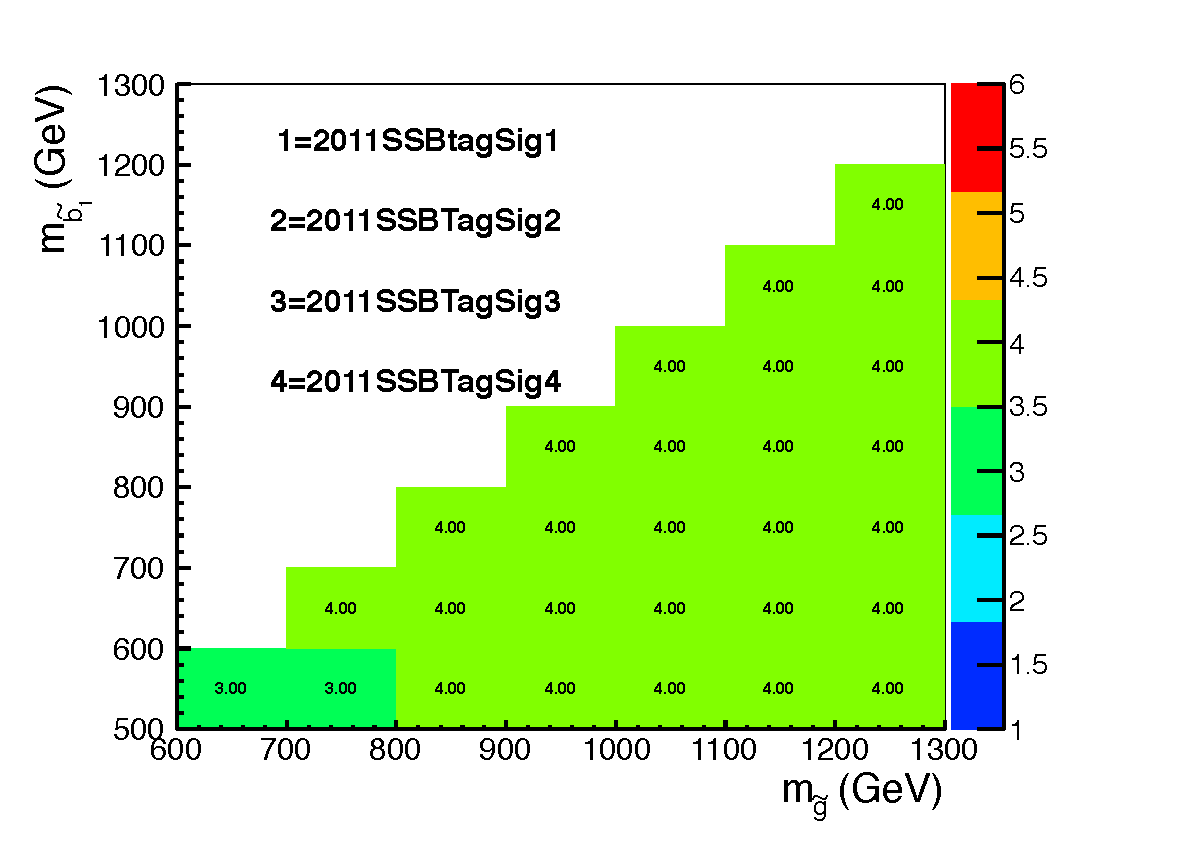
\includegraphics[width=0.65\linewidth]{figs/gl_sb_300_50_regions.pdf}
\caption{The signal region with the best expected limit as a function of 
$m(\widetilde{g})$ vs. $m(\widetilde{b})$ for $m(\chi^0_1)$=50 GeV
and $m(\chi^{\pm})$=200 GeV. 
The coding is: 1=(200-50), 2=(200-150), 3=(320-50), and 4=(320-120), where
the first (second) number is the $H_T$ (\met) threshold in GeV. The number
of requested btags is 2 or more.
\label{fig:gluinosboptimize}}
\end{center}
\end{figure}


For each point in parameter space we use the signal region that gives
the best expected limit.  
{\bf (Note: so far the region with 3 btags has not been used).}
Limits are calculated using all experimental
uncertainties; the JES and btag uncertainties are calculated point-by-point.
An example of this optimization is shown in Figure~\ref{fig:gluinosboptimize},
where we show the choice of signal region that gives the best expected limit
in the $m(\widetilde{g})$ vs. $m(\widetilde{b})$ plane for the choice
$m(\chi^0_1)$=50 GeV and $m(\chi^{\pm})$=200 GeV. 
Roughly speaking we we exclude gluino masses below about 750 GeV for 
all sbottom masses kinematically accessible, {\it i.e.}, 
$m(t)+m(\chi^{\pm})~<~m(\widetilde{b})~<~m(\widetilde{g})$.



\subsubsection{Limits for the $\widetilde{g} \to \widetilde{b}b$ Model}
\label{sec:gbblimits}

The limits on the production cross-section in this model in the 
gluino mass vs. sbottom mass plane for two choices of the 
chargino mass and an LSP mass of 50 GeV 
are shown in Figure~\ref{fig:mglinoSbottom}
Using the 
NLO$+$NLL cross-section for gluino pair production, we also place a limit
on the mass parameters of this model.


\begin{figure}[htb]
\begin{center}
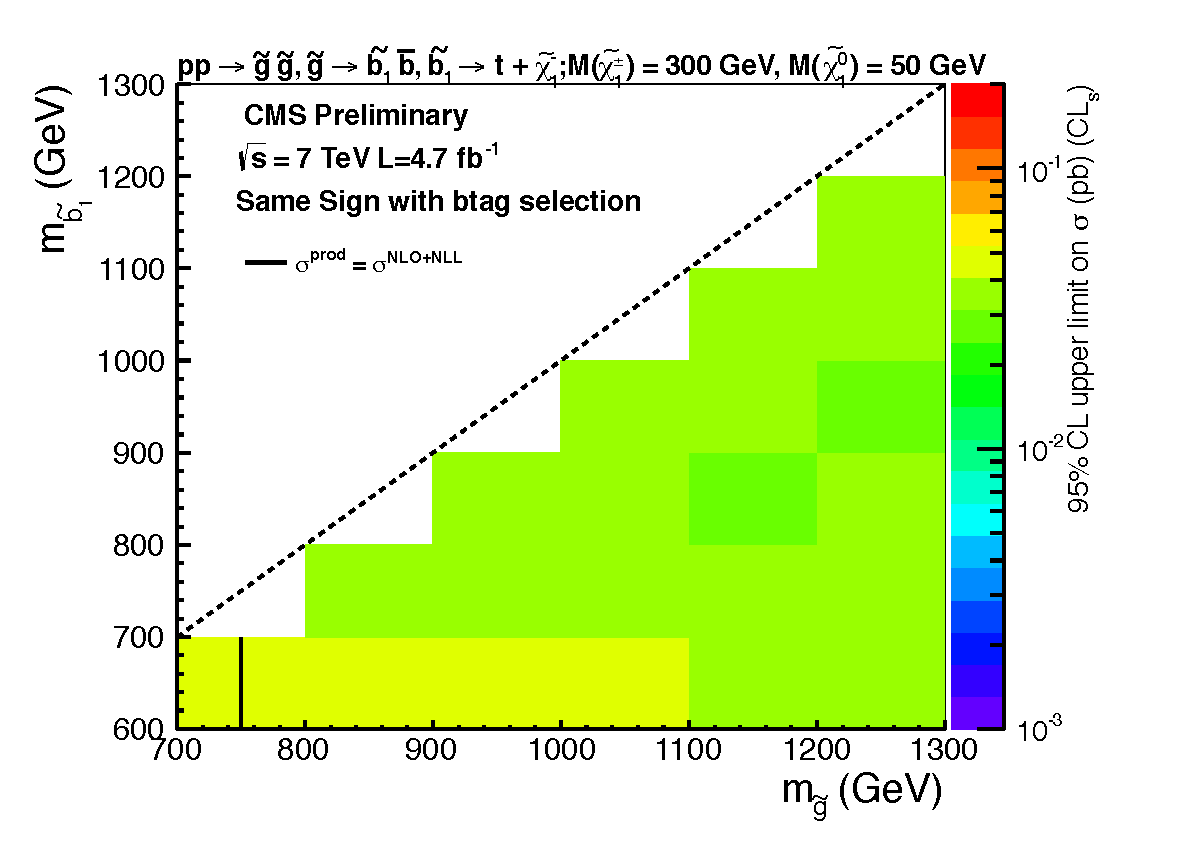
\includegraphics[width=0.47\linewidth]{figs/gl_sb_300_50.pdf}
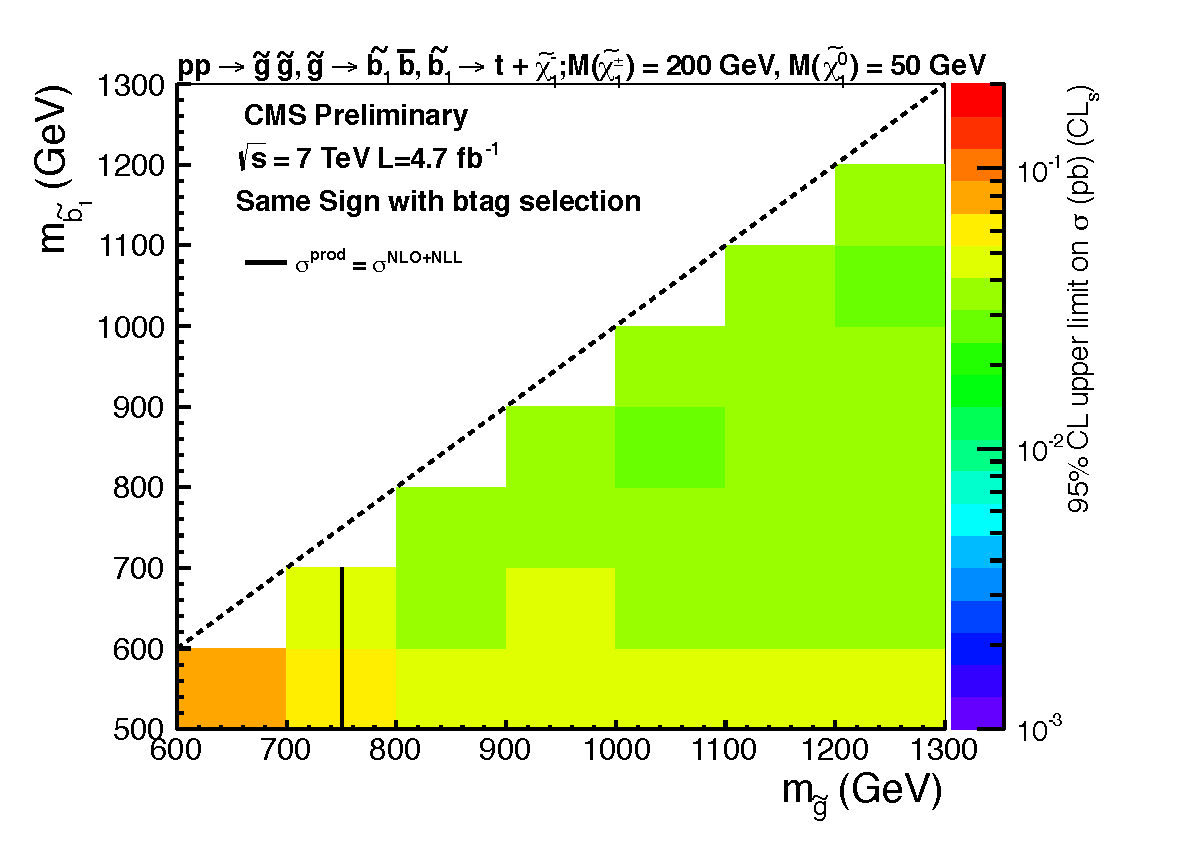
\includegraphics[width=0.47\linewidth]{figs/gl_sb_200_50.pdf}
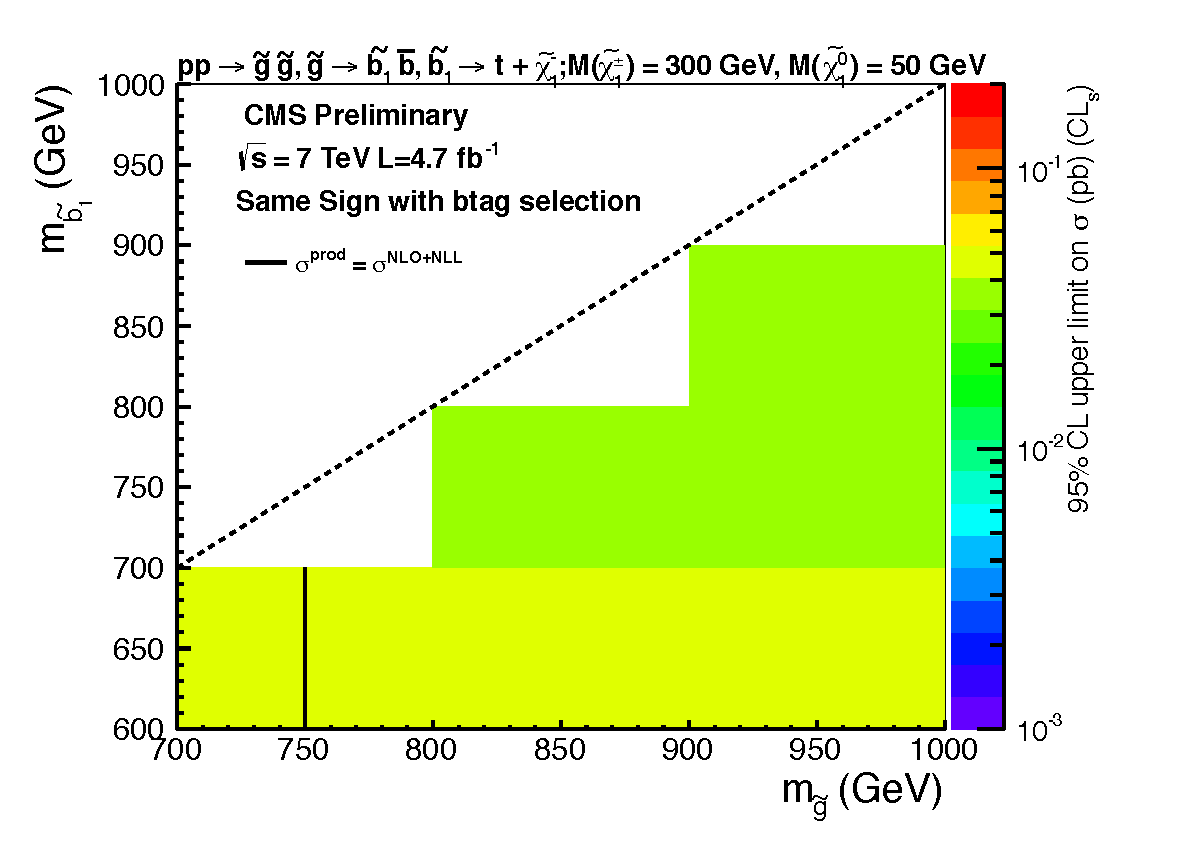
\includegraphics[width=0.47\linewidth]{figs/gl_sb_300_50_zoom.pdf}
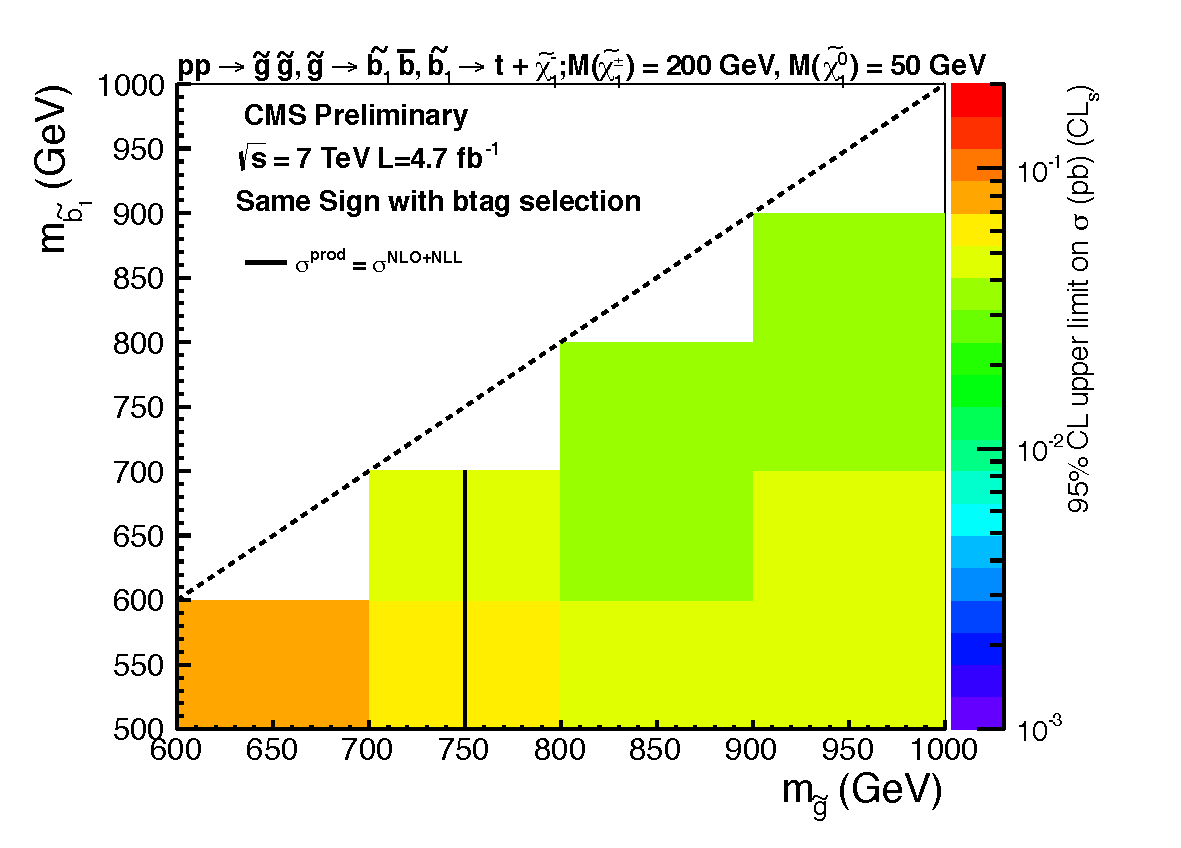
\includegraphics[width=0.47\linewidth]{figs/gl_sb_200_50_zoom.pdf}
\caption{Cross section limits in the $m(\widetilde{g})$ vs. 
$m(\widetilde{b})$ plane
for $m(\chi_1^0)$ = 50 GeV and 
$m(\chi^{\pm})$ = 300 GeV (left) and 200 GeV (right). 
The bottom plots are ``zoomed'' in versions of the top plots.
\label{fig:mglinoSbottom}}
\end{center}
\end{figure}

%\subsubsection{What is missing for the $\widetilde{g} \to \widetilde{b}\bar{b}$ Model}
%\begin{itemize}
%\item Everything in Sections~\ref{sec:gbbdefinition} and \ref{sec:gbblimits}
%\item It would be nice to have a reference.  I am not sure that the 
%references that
%we have on our twiki are appropriate. 
%\item Perhaps more details on the MC signal generation
%\end{itemize}



\subsection{Additional SUSY plots}
\label{sec:moreSUSYplos}

{\bf Impotant: Many of the plots here and in the previous Sections
need to be prettified.  Also: in some cases we are in the
process of adding scan points with parameters near the limit 
lines to get more meaningful plots.}


In this Section we collect additional SUSY plots.  These are 
candidate plots for the public {\tt twiki} page and/or the 
journal publication.

Figure~\ref{fig:gluinoLimit1d} shows the gluino mass limits
in the models with gluino-pair production considered here.
Not surprisingly,
we find that the gluino mass limit is fairly insensitive 
to the details of the decay chain, since the limit
is drien by the gluino ross-section.

Figure~\ref{fig:stoppaper} is a candidate Figure for inclusion
in a publication to summarize the limits on models 
with real or vitual stops.
Similarly, Figure~\ref{fig:sbottompaper} is a candidate Figure for inclusion
in a publication to summarize the sbottom limits.



\begin{figure}[htb]
\begin{center}
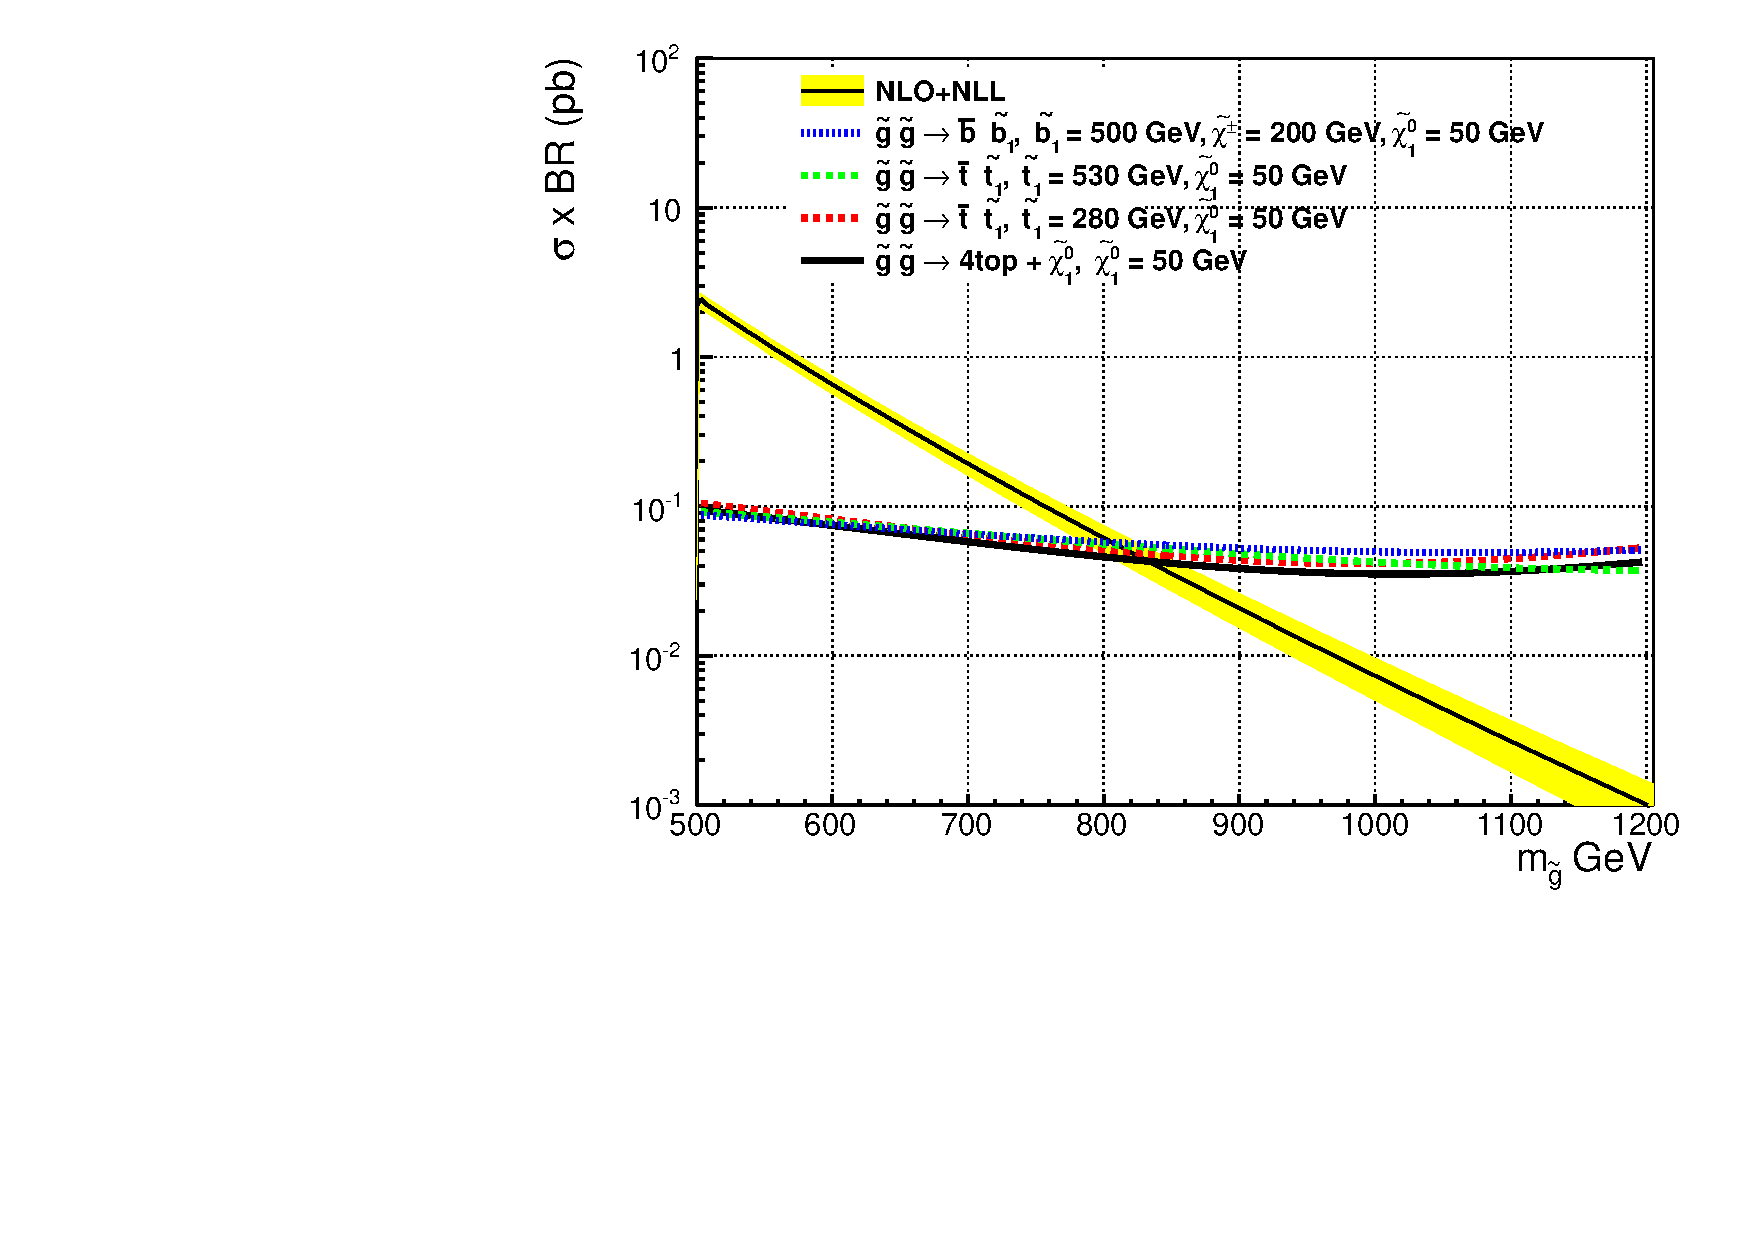
\includegraphics[width=0.48\linewidth]{figs/gluino_1d.pdf}
\caption{Gluino pair-production cross-section
as a function of gluino mass compared with limits
on the cross-section from the models considered here.
\label{fig:gluinoLimit1d}}
\end{center}
\end{figure}





\begin{figure}[bht]
\begin{center}
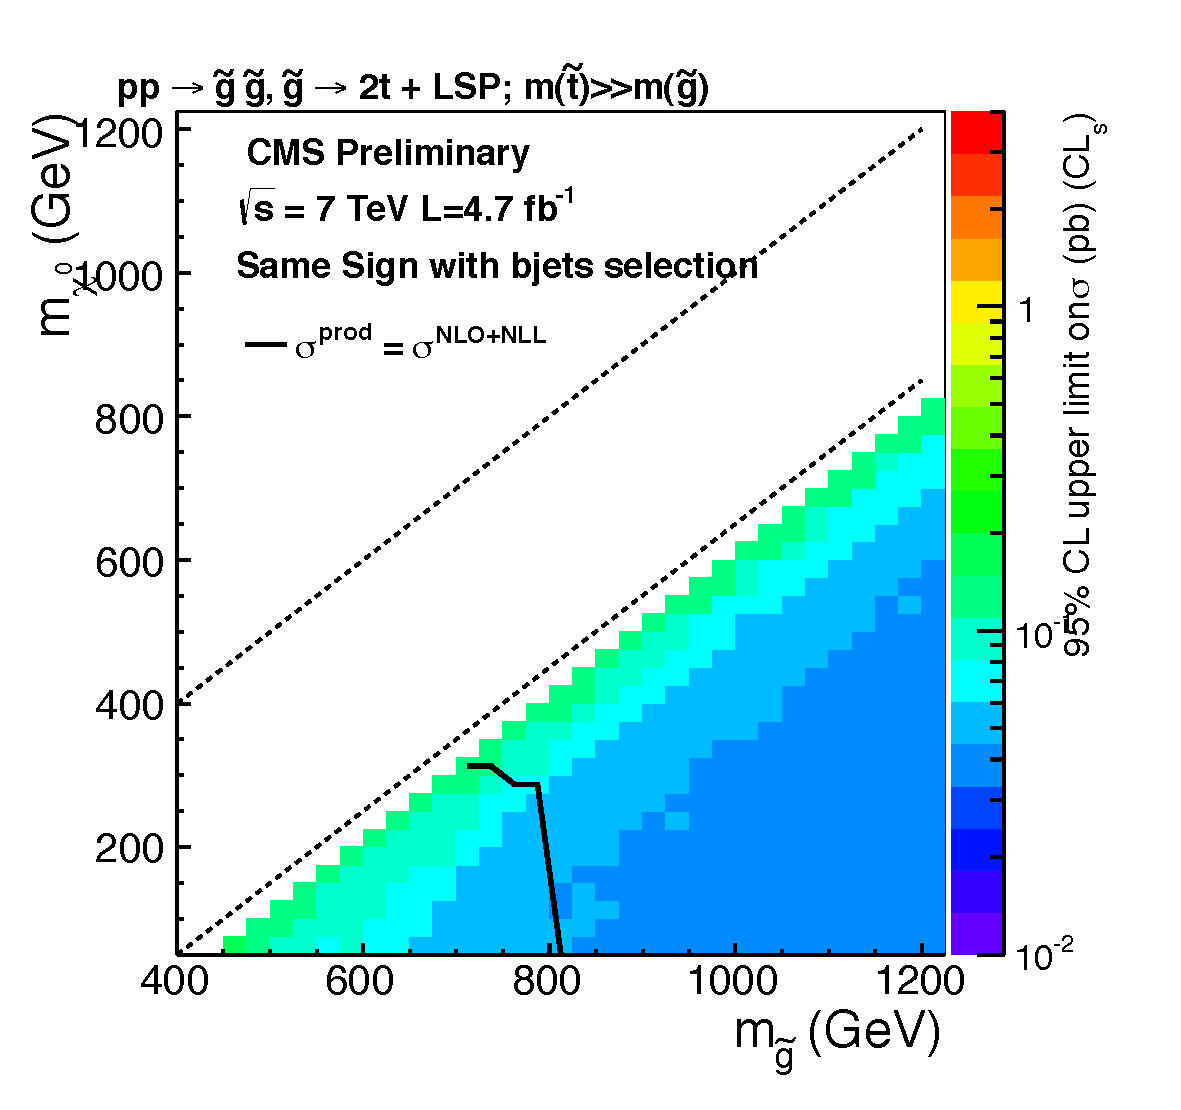
\includegraphics[width=0.49\linewidth]{figs/T1tttt.pdf}
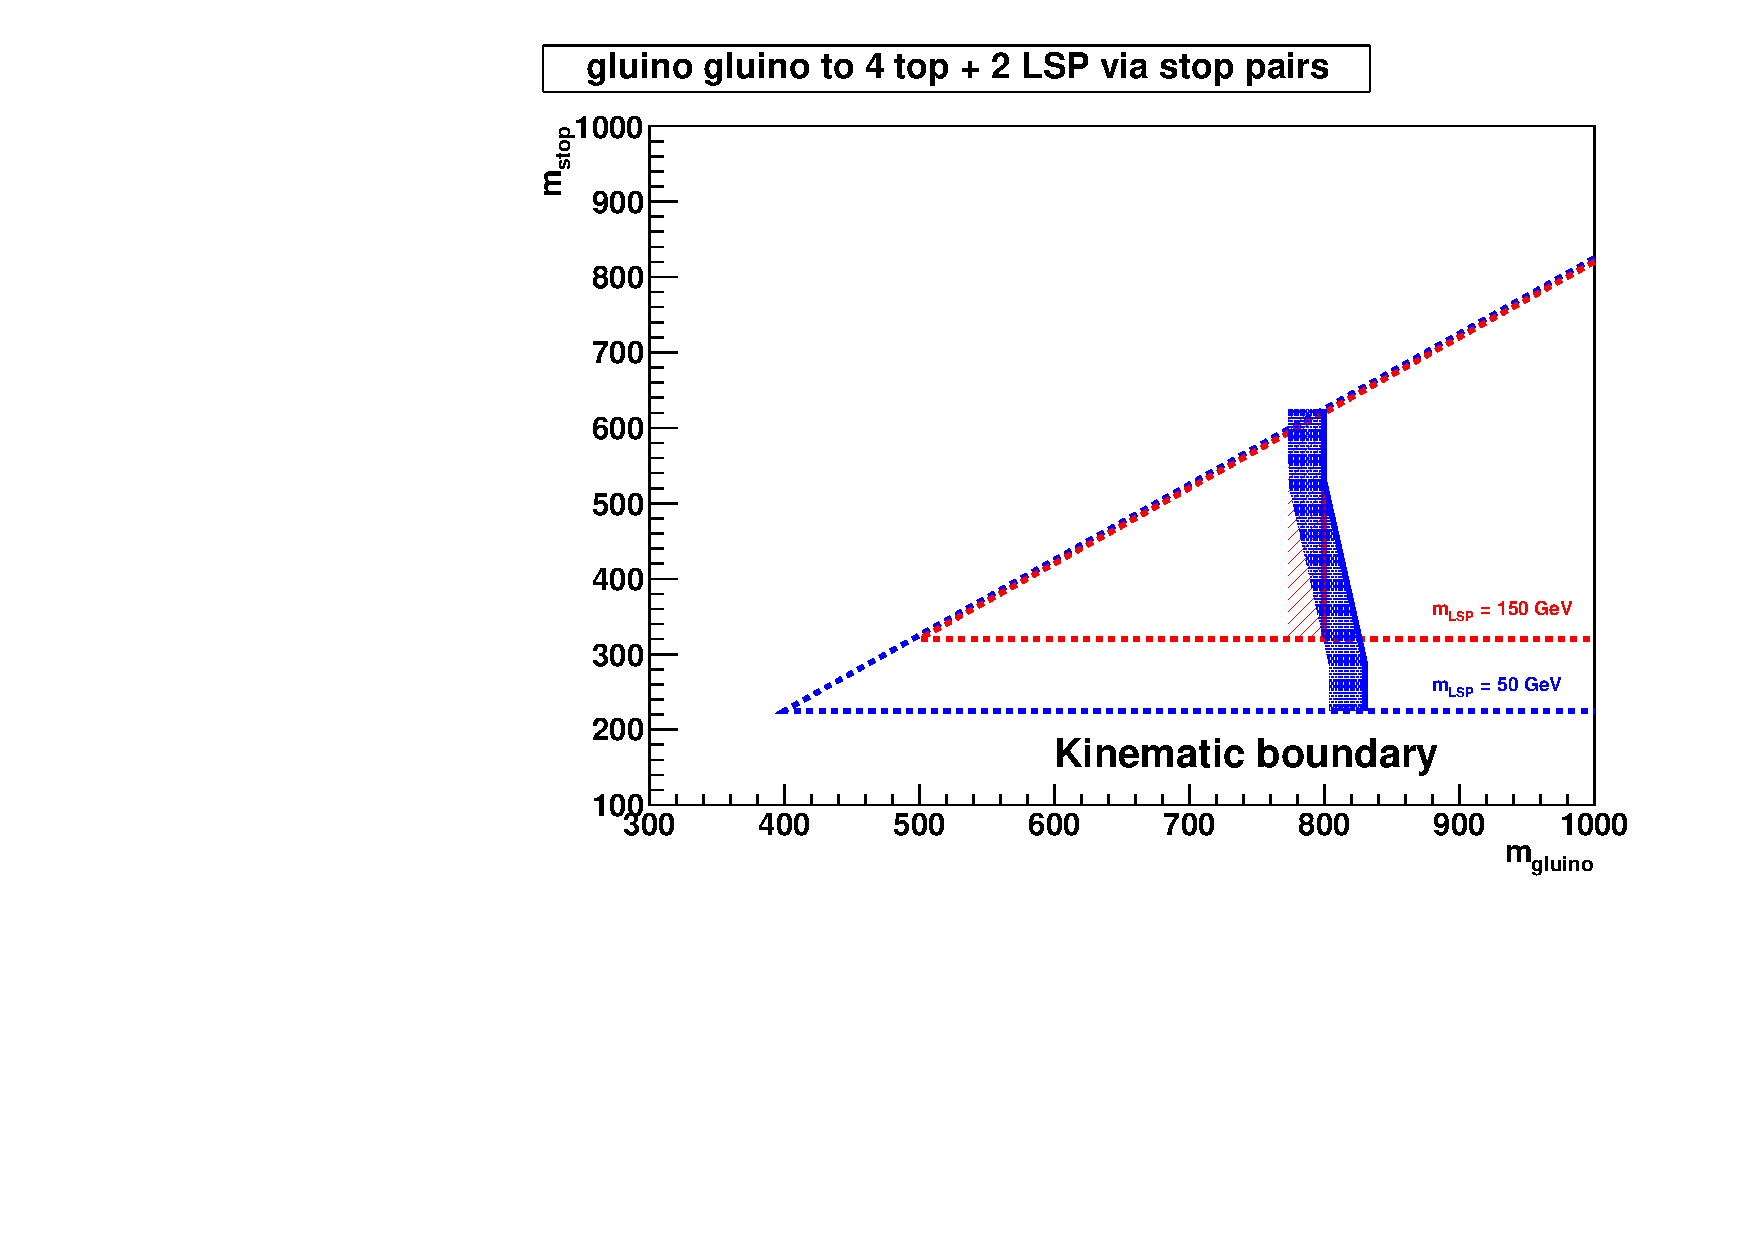
\includegraphics[width=0.49\linewidth]{figs/gluinoStop_fkw}
\caption{Left plot: exclusion contour (95 \% C.L.) in the 
$m(\chi^0_1)-m(\widetilde{g})$ 
plane for model with gluino decay via virtual stop quarks.
Right: exclusion contours (95 \% C.L.) in the 
$m(\widetilde{t})-m(\widetilde{g})$
plane for model wih gluino decay to on-shell top squarks)
for different choices of the LSP mass.  
{\bf We need to get rid of the temperature plot for the
left plot.  The right plot needs a lot of work...
The blue and the red lines show the allowed
kinematical regions for LSP masses of 50 and 150 GeV,
respectively.  The dots represents the boundaries of 
the exclusion region.  The placement of the dots needs 
to be refined, the dots need to extend a bit closer to
the boundary, the dots should be joined by a line.} 
\label{fig:stoppaper}}
\end{center}
\end{figure}


\begin{figure}[thb]
\begin{center}
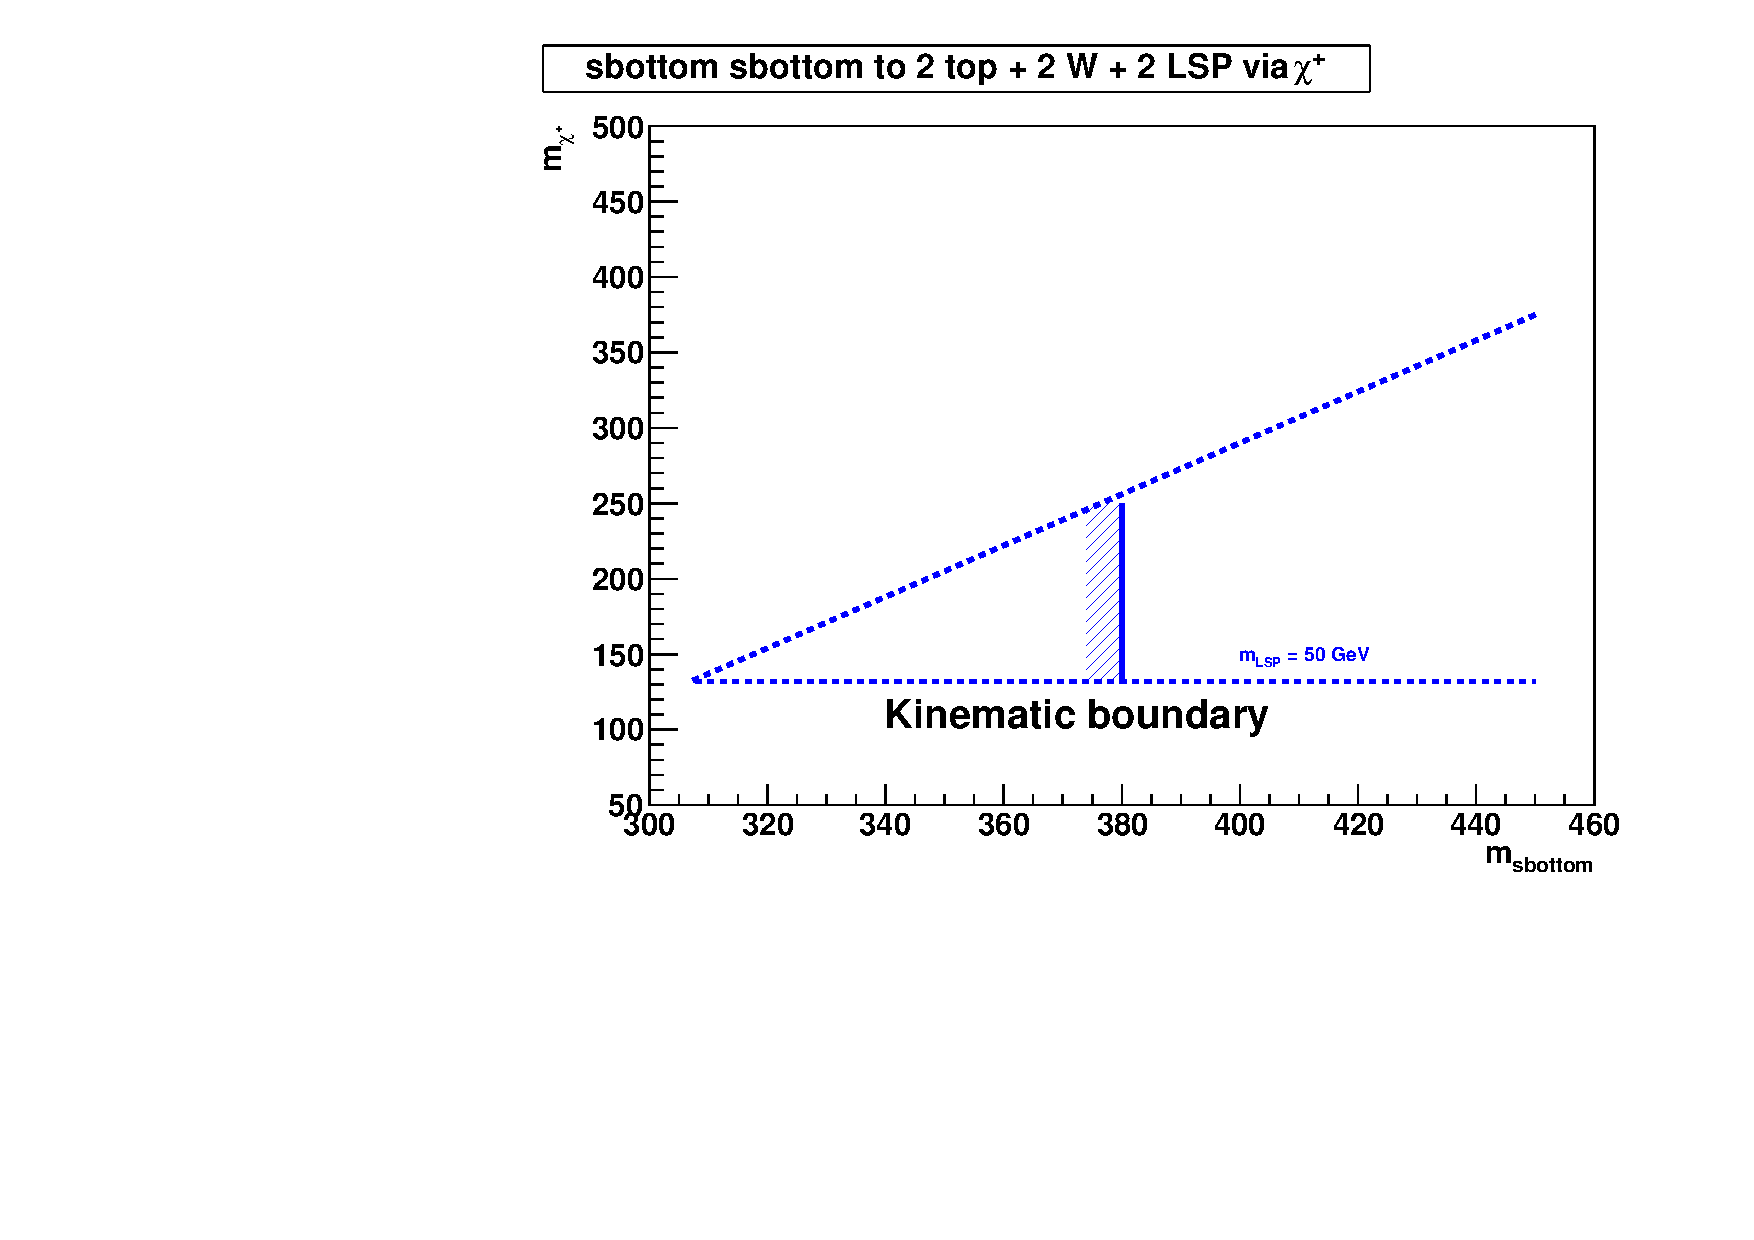
\includegraphics[width=0.49\linewidth]{figs/sbottom_fkw.pdf}
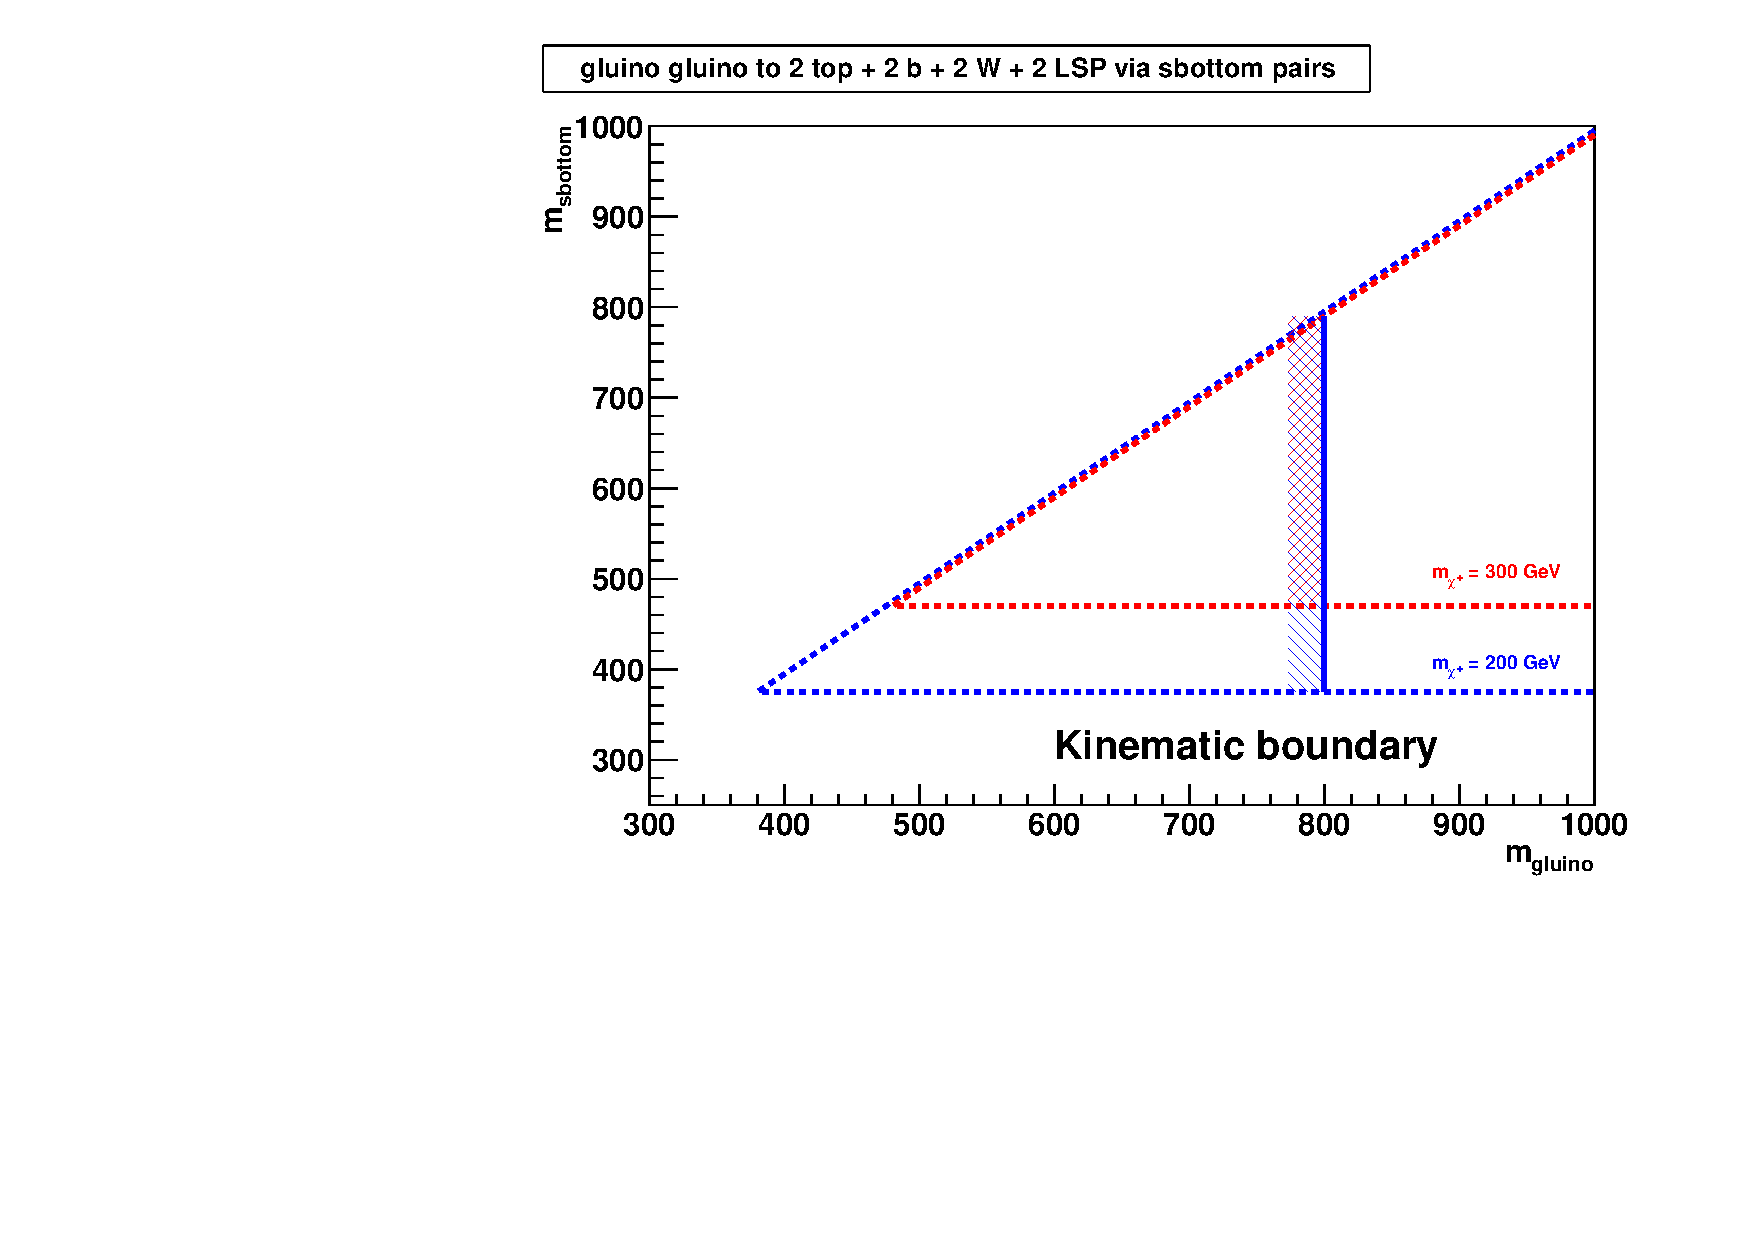
\includegraphics[width=0.49\linewidth]{figs/gluinoSbottom_fkw.pdf}
\caption{(a) 
Exclusion contour (95 \% C.L.) in the 
$m(\chi^{-})-m(\widetilde{b})$ 
plane for the sbottom pair production model; 
(b) Exclusion contours (95 \% C.L.) in the $m(\widetilde{b})-m(\widetilde{g})$
plane for model with sbottom production from gluino decay).
{\bf Plots need work.  Of course, labels, etc. 
Left plot needs more points, better point placement, a line joining them.
Right plots: the blue (red) line show the kin limits for m(chargino)=200 (300)
and m(LSP)=50.  The points need better placement, more points, a line going 
through them} 
\label{fig:sbottompaper}}
\end{center}
\end{figure}




\clearpage
